%% ----------------------------------------------------------------
%% CapSizing.tex
%% ----------------------------------------------------------------

\graphicspath{{CapSizing/figure/}}

\chapter{Exploring the Effect of Energy Storage Sizing on Intermittent Computing System Performance}

Batteryless energy-harvesting devices promise to deliver a sustainable Internet of Things. Intermittent computing is an emerging area, where forward progress of application execution is maintained by saving volatile computing state into non-volatile memory before power interruptions, and restored afterwards. Conventional intermittent computing approaches typically minimize energy storage to reduce device dimensions and interruption periods, 
but this can result in high state-saving and -restoring overheads and impede forward progress. 
In this paper, we argue that adding a small amount of energy storage can significantly improve forward progress. 
We develop an intermittent computing model that accurately estimates forward progress, with an experimentally validated mean error of 0.5\%. 
Using this model, we show that sizing energy storage can improve forward progress by up to 65\% with a constant current supply, and 43\% with real-world photovoltaic sources. 

An extension to this approach, which uses a cost function to trade off the energy storage size against forward progress, can save 83\% of capacitor volume and 91\% of interruption periods while maintaining 93\% of the maximum forward progress.

\section{Introduction}

% *** Background of energy harvesting and intermittent systems ***

%Energy harvesting has become a promising power solution for the Internet of Things, liberating wireless sensors from batteries and the power grid~\cite{sliper2020energy-driven}. 
%Batteryless devices harvest ambient energy, such as light, radio-frequency, and mechanical vibration~\cite{sravanthi2008survey, shaikh2016energy}, which is then buffered in a capacitor. 
%As the harvested power is typically insufficient for continuous operation, such devices operate in an intermittent way -- when a certain amount of energy is collected, the processor wakes up, executes program until the amount of energy falls below a threshold, where it sleeps or dies, and waits for the next active cycle\footnote{An active cycle denotes a continuous period that the intermittent system actively executes workloads, i.e. from when it wakes up till it dies or sleeps. }. 
%Prior work in \textit{intermittent systems} has developed sophisticated methods to preserve forward progress across frequent power interruptions by carefully \textit{checkpointing} the volatile computing state in CPU registers and volatile memory into non-volatile memory (NVM), and restoring the state after power interruptions~\cite{umesh2021survey}. 


% *** Previous work on intermittent peripheral operations ***

Apart from computing, embedded sensor systems need to utilize peripherals, such as sensors, computational accelerators, and radios, which typically require \textit{atomicity}~\cite{berthou2020formal}.
In the context of IPSs, an atomic operation should not be checkpointed during execution; if interrupted by power failures, it should restart rather than checkpoint and resume.
% A peripheral operation is considered atomic because it is infeasible to completely read, save, and restore the intermediate internal state of peripherals, and even if possible, could produce unwanted results (e.g. violating timeliness). 
A peripheral operation is considered atomic because it is usually problematic to checkpoint and restore the operation later, even if the intermediate peripheral state is also checkpointed.
For example, checkpointing during a sensor reading and resuming it later can cause incorrect results or an infinite wait as the initialization is lost, and violate timeliness as the sensor does not render the latest and consecutive results~\cite{maeng2019supporting}. 
% disable checkpoints during execution
Prior works on intermittent peripheral operations either customize a design-time calibrated energy budget for each peripheral operation individually~\cite{gomez2016dynamic}, or allocate a universal and large energy budget that ensure the most energy-hungry operation can finish in one active cycle~\cite{maeng2019supporting}.




% *** Offline profiling and fixed threshold is impractical due to variability ***

However, in this paper we argue that manually profiling each peripheral operation and customizing energy thresholds is impractical due to variability in intermittent systems, where we have considered the variability in the data amount to process, peripheral configurations, devices, and energy buffering capacitance (detailed in Section~\ref{subsec:dynamic_energy_consumption}). 
A fixed threshold can be violated if any of the above cases happen, and lead to non-termination\footnote{Non-termination happens when the pre-defined energy budget is less than how much the operation consumes and the supply is not strong enough to fill the energy gap. It is one of the main causes for failures in intermittent systems. }.
In practical deployment, considering the complexity and labour effort, it is unrealistic to profile every atomic operation for every device under every runtime scenario at design time and customize the energy budgets accordingly. 



% *** An optimized threshold improves efficiency ***

On the other hand, using only one high voltage threshold, though probably avoids non-termination, can affect system energy efficiency. 
% Microcontrollers and peripheral devices typically draw more current at a higher supply voltage. 
Intermittent systems typically minimize operating voltage in order to lower quiescent power consumption from power conversion loss and system leakage~\cite{gomez2016dynamic}. 
Also, a high operating voltage can decrease the output current of energy harvesters, making it harder to charge up the buffering capacitor~\cite{pan2017maximize}.
Hence, setting a high wake-up voltage threshold results in a superlinear long charging time, which therefore slows down the system execution or even leave the system in an infinite wait at low input power.
% \todo{Illustrate or demonstrate this?}


% *** What we do to address it ***

To address the above issue, we propose \nn{}\footnote{\nn{}: \underline{O}nline Energy \underline{P}rofiling and \underline{T}hreshold Adaptation for \underline{I}ntermittent \underline{C}omputing Systems. }, a methodology that profiles energy consumption of operations at runtime and dynamically adapts energy thresholds based on newly profiled consumption and user-defined parameters. 
A naive approach of runtime energy profiling can be disconnecting the power supply during profiling and taking two readings of supply voltage before and after an operation~\cite{zhan2020adaptive}, but this can waste the harvested energy during the operation. 
In contrast, \nn{} profiles the maximum drop of supply voltage that an operation can cause while the energy harvesting supply is connected. 
The profiling strategy is to measure the input current in the charging cycle so as to calculate the maximum drop of supply voltage in the discharging cycle. 
The runtime profiled energy budget can closely match the latest energy consumption of an atomic operation. 
Based on the profiling results, \nn{} dynamically adapts the threshold for each atomic operation, with an option of scaling threshold by user-defined parameters or peripheral configurations.
Therefore, \nn{} avoids non-termination and achieves high energy efficiency, improving the workload throughput.

The main contributions of this article are as follows:

\begin{enumerate}
    \item Design exploration (Section~\ref{sec:design_exploration})
    \item Methodology (Section~\ref{sec:method1} and Section~\ref{sec:method2})
    \item Implementation (Section~\ref{sec:implementation})
    \item Experimental evaluation (Section~\ref{sec:experiment})
\end{enumerate}
\input{CapSizing/review2}
%%%%%%%%%%%%%%%%%%%%%%%%%%%%%%%%%%%%%%%%%%%%%%%%%%%%%%%%%%
%%% Section 3: Modelling Reactive
%%%%%%%%%%%%%%%%%%%%%%%%%%%%%%%%%%%%%%%%%%%%%%%%%%%%%%%%%%

\section{Reactive ICS Modelling} \label{section:model}

% The goal of this model is to facilitate making design decisions when deploying intermittent computing devices in real-world environments by enabling designers to observe how the sizes of energy harvester and energy storage have an impact on the key design specifications, i.e. forward progress, dimensions, and interruption periods.

% We then illustrate a formulation which describes the relationship between forward progress and energy storage capacitance given different harvested power level in reactive intermittent computing as a part of the exploration model. 

% Assumptions. low variation in harvested power, how low? what's the impact of high variance input?
% given a constant current supply
To facilitate the understanding and exploration of reactive ICSs, we present a model which outputs the normalized forward progress $\alpha_{exe}$ when powered from a constant current supply $I_{harv}$. Parameters of this model are listed in Table~\ref{tab:parameter}. 
%This accounts for the \textit{Energy Storage} and \textit{Intermittent Load} modules in the system model, allowing the expected forward progress to be evaluated.
% The input parameters $I_{harv}$ and $C$ are related to the size configuration of energy harvester and energy storage respectively. 
% for a period of time that long enough to omit an individual uncompleted operating cycle. 
The model assumes that all configuration parameters remain constant. 

\begin{table}[!t]
    \renewcommand{\arraystretch}{1.2}
    \centering
    \caption{Model parameters of reactive ICS} 
    \label{tab:parameter}
    % Some packages, such as MDW tools, offer better commands for making tables
    % than the plain LaTeX2e tabular which is used here.
    \begin{tabular}{|c|c|}
        % \hline
        % \textbf{Parameter} & \textbf{Description} \\
        \hline
        \multicolumn{2}{|c|}{\textbf{Input Parameters}}\\
        \hline
        $I_{harv}$ & Energy harvester current supply\\
        $C$ & Energy storage capacitance\\
        \hline
        \multicolumn{2}{|c|}{\textbf{Configuration Parameters}}\\
        \hline
        $I_{exe}$ & Execution current draw\\
        $I_{lpm}$ & Low-power mode current draw\\
        %$I_{load}$ & Total current draw of load\\
        $I_{r}$ & Restore current draw\\
        $I_{s}$ & Save current draw\\
        $I_{leak}$ & Leakage current draw\\
        $V_{r}$ & Restore voltage threshold\\
        $V_{s}$ & Save voltage threshold\\
        $T_{r}$ & Restore time overhead\\
        $T_{s}$ & Save time overhead\\
        \hline
        \multicolumn{2}{|c|}{\textbf{Output Parameter}}\\
        \hline
        $\alpha_{exe}$ & Normalized forward progress \\ 
        \hline
    \end{tabular}
\end{table}

% Since supply current $I_{harv}$ and leakage current $I_{leak}$ constantly exist (though could be zero), 
For brevity, $I_{in}$ denotes the usable input current as expressed in (\ref{eq:in}). The effect of capacitor leakage current, $I_{leak}$, is discussed at the end of Section~\ref{subsec:formulation}.
\begin{equation}
  I_{in} = I_{harv} - I_{leak}
  \label{eq:in}
\end{equation}

\subsection{Operating Modes of Reactive ICS}

The behavior of reactive ICSs can be classified into three operating modes depending on the supply current, as shown in \figurename{~\ref{fig:operatingModes}}. These are differentiated by the relationship between input current $I_{in}$ and the system's current draw in its low-power mode (LPM) or active modes, i.e. $I_{lpm}$ and $I_{exe}$. We define the three modes as:

\begin{figure}[!t]
  \centering
  \includegraphics[width=3.2in]{ch3_sizingeffect/figures/OperatingMode0Fig}
  \caption{Operating modes of reactive ICSs, and achieved forward progress against supply current.}
  \label{fig:operatingModes}
\end{figure}

\begin{itemize}
	\item \textit{Off} mode: When $I_{in} < I_{lpm}$, the system stays inactive. The supply voltage $V_{cc}$ cannot rise above the restore threshold $V_{r}$ to wake the system and start execution. The LPM current $I_{lpm}$ includes the consumption of voltage monitoring circuits and system idle current.
	% Here, $I_{lpm}$ is induced after $V_{cc}$ goes above the minimum operating voltage $V_{off}$ where the system waits for $V_{cc}$ to reach $V_{r}$ (when $V_{off} < V_{cc} < V_{R}$). 

    \item \textit{On} mode: When $I_{in} > I_{exe}$, the system executes constantly as the supply voltage $V_{cc}$ never drops below $V_{s}$. $V_{cc}$ grows until $I_{in}$ and $I_{exe}$ are in equilibrium, which may result from $I_{in}$ decreasing due to poor impedance matching, or $I_{exe}$ increasing due to either greater current draw at higher voltage or dissipation through overvoltage protection circuits. 

	\item \textit{Intermittent} mode: When $I_{lpm} < I_{in} < I_{exe}$, the system executes intermittently after $V_{cc} > V_{r}$ and before $V_{cc} < V_{s}$. $V_{cc}$ can rise above $V_{r}$ and the system starts execution. However, the stored energy is then consumed by the load as $I_{in} < I_{exe}$, causing $V_{cc}$ to eventually drop below the save threshold $V_{s}$, where the system saves its state and enters LPM. The system stays in LPM until $V_{cc}$ rises to $V_{r}$ again and then resumes execution. 
	% In this mode, $V_{cc}$ oscillates approximately between $V_{r}$ and $V_{s}$, 'switching' on and off the execution. 
    In general, a higher $I_{in}$ leads to more forward progress in this mode, but the exact relationship between $I_{in}$ and forward progress requires further analysis.
    
	% The excess power either dissipates through circuits or overcharges $V_{cc}$. An overcharged $V_{cc}$ may affect harvesting efficiency due to poor impedance matching and reduce $I_{harv}$, such that current input and consumption are in equilibrium. 
	% In this model case, charging $V_{cc}$ above the maximum power point of the PV cell reduces $I_{harvest}$, and $V_{cc}$ is stable when $I_{harvest} = I_{exe} + I_{leak}$. 
\end{itemize}

\subsection{Formulating Forward Progress} \label{subsec:formulation}

Next, we derive formulations to calculate $\alpha_{exe}$ from $I_{in}$ and energy storage capacitance $C$. We then explore the effect of capacitor leakage on maximum forward progress. 

In the \textit{On} and \textit{Off} modes, the normalized forward progress is trivial to find (simply 1 and 0 respectively). In the \textit{Intermittent} mode,  as shown in \figurename{~\ref{fig:operatingCycle}}, the system goes through four intervals in turn, i.e. charging, restoring, executing, and saving, with current consumption of $I_{lpm}$, $I_{r}$, $I_{exe}$, and $I_{s}$ in each interval respectively. The normalized forward progress, i.e. effective execution time ratio, is indicated as $T_{exe} / T_{cycle}$, where $T_{exe}$ is the time spent on effective execution in one operating cycle and $T_{cycle}$ is the period of operating cycles. Hence, the forward progress given all supply levels is expressed as:
\begin{equation}
    \alpha_{exe} = \left\{
    \begin{aligned}
        & 0 & , & \quad \textit{Off} \, (I_{in} < I_{lpm}) \\
        & \frac{T_{exe}}{T_{cycle}} & , & \quad \textit{Intermittent} \, (I_{lpm} < I_{in} < I_{exe}) \\
        & 1 & , & \quad \textit{On} \, (I_{in} > I_{exe})
    \end{aligned}
    \right.
    \label{eq:feff}
\end{equation}

\begin{figure}[!t]
  \centering
  \includegraphics[width=3.33in]{ch3_sizingeffect/figures/CRESdemoFig}
  \caption{Operating cycles in the \textit{Intermittent} mode. }
  \label{fig:operatingCycle}
\end{figure}

In the following analysis, we focus on deriving $T_{exe} / T_{cycle}$ in the \textit{Intermittent} mode. Let $V_{pr}$ (post-restore) and $V_{ps}$ (post-save) denote the voltage after restoring and saving operations. $V_{pr}$ and $V_{ps}$ can be calculated as:
\begin{equation}
  V_{pr} = V_{r} + \frac{T_{r} (I_{in} - I_{r})}{C}
  \label{eq:vpr}
\end{equation}
\begin{equation}
  V_{ps} = V_{s} + \frac{T_{s} (I_{in} - I_{s})}{C}
  \label{eq:vps}
\end{equation}
With (\ref{eq:vpr}), the time spent on effective execution $T_{exe}$ in one operating cycle can be expressed as:
\begin{equation}
%   \begin{aligned}
    T_{exe} = \frac{C(V_{pr} - V_{s})}{I_{exe} - I_{in}} 
    % & = \frac{C(V_{r} - V_{s}) + T_{r} (I_{in} - I_{r})} {I_{exe} - I_{in}}
%   \end{aligned}
  \label{eq:texe}
\end{equation}
Analogously, with (\ref{eq:vps}), the charging interval can be described as:
\begin{equation}
%   \begin{aligned}
    T_{charge} = \frac{C(V_{r} - V_{ps})}{I_{in} - I_{lpm}}
    % & = \frac{C(V_{r} - V_{s}) - T_{s} (I_{in} - I_{s})} {I_{in} - I_{lpm}}
%   \end{aligned}
  \label{eq:tcharge}
\end{equation}
With (\ref{eq:texe}) and (\ref{eq:tcharge}), the period of an operating cycle is:
\begin{equation}
%   \begin{aligned}
    T_{cycle} = \quad T_{charge} + T_{r} + T_{exe} + T_{s} 
%     = & \quad \frac{C (V_{r} - V_{s}) + T_{s} (I_{s} - I_{lpm})}{I_{in} - I_{lpm}} \quad + \\
%     & \quad \frac{C (V_{r} - V_{s}) + T_{r} (I_{exe} - I_{r})}{I_{exe} - I_{in}}
%   \end{aligned}
  \label{eq:tperiod}
\end{equation}

Finally, combining (\ref{eq:vpr})--(\ref{eq:tperiod}), we obtain normalized forward progress $\alpha_{exe}$ in the \textit{Intermittent} mode as:
\begin{equation}
    \begin{aligned}
        \alpha_{exe} &= \frac{T_{exe}}{T_{cycle}} \\ %, \quad I_{lpm} < I_{in} < I_{exe}
                     &= \frac{\frac{C (V_{r} - V_{s}) + T_{r} (I_{in} - I_{r})} {I_{exe} - I_{in}}}{\quad \frac{C (V_{r} - V_{s}) + T_{s} (I_{s} - I_{lpm})}{I_{in} - I_{lpm}} + \frac{C (V_{r} - V_{s}) + T_{r} (I_{exe} - I_{r})}{I_{exe} - I_{in}}} \\
                    %  &= \frac{\scriptstyle \bigl[C (V_{r} - V_{s}) + T_{r} (I_{in} - I_{r}) \bigr] (I_{in} - I_{lpm})}{\scriptscriptstyle C (V_{r} - V_{s}) (I_{exe} - I_{lpm}) + T_{s} (I_{in} - I_{s}) (I_{exe} - I_{in}) + T_{r} (I_{exe} - I_{r}) (I_{in} - I_{lpm})} \\
    \end{aligned}
    \label{eq:texepercent}
\end{equation}
In the numerator $T_{exe}$, $C(V_{r} - V_{s})$ represents the amount of charge in the capacitor available for restoring and executing. $T_{r} (I_{in} - I_{r})$ represents the charge used by a restore operation. $I_{exe} - I_{in}$ is the rate of charge consumption from the energy storage during execution.

% \footnote{Calculation breakdowns of differential analysis is attached in Appendix.}
% Higher $\alpha_{exe}$ leads to more time spent on forward progress. 

% As $d\alpha_{exe} / dI_{in}$ is positive, higher harvested current $I_{harv}$ leads to more forward progress. 
To explore the effect of energy storage on forward progress, we need to analyze $d\alpha_{exe} / dC$. Here, if we assume that $I_{leak}$ remains constant, $\alpha_{exe}$ keeps increasing and approaches $(I_{in} - I_{lpm}) / (I_{exe} - I_{lpm})$ when energy storage capacitance $C$ increases. Defining $(I_{in} - I_{lpm}) / (I_{exe} - I_{lpm})$ as $\alpha_{exe\_ideal}$, $\alpha_{exe} = \alpha_{exe\_ideal}$ is an ideal case, where restore and save overheads are absent.

In an electrolytic capacitor, however, $I_{leak}$ typically increases with $C$ with the following relationship~\cite{avxleakage}:
\begin{equation}
    I_{leak} = kCV_{cc}
    \label{eq:ileak}
\end{equation}
where $k$ is a constant normally in a range 0.01 to 0.03 ($\frac{A}{F \cdot V}$). Combining (\ref{eq:ileak}) with (\ref{eq:in}), $dI_{in} / dC$ is $-kV_{cc}$, meaning $I_{in}$ decreases linearly as $C$ increases. Thus, when $C$ increases, $\alpha_{exe}$ keeps approaching $\alpha_{exe\_ideal}$ while $\alpha_{exe\_ideal}$ decreases. Hence, we believe that there is a capacitance value that leads to the maximum $\alpha_{exe}$ considering $I_{leak}$ increases with $C$.
% \cite{alcapacitor}
% Also, the time overhead of state saving and restoring operations $T_{RS\%}$ can be calculated as:
% \begin{equation}
%   T_{RS\%} = \frac{T_{R} + T_{S}}{T_{exe} + T_{R} + T_{S}}
% \end{equation}


% In Equation~(\ref{eq:feff}), we get the relationship between forward progress and the sizes of energy harvester and energy storage. 

\section{Experimental Evaluation} \label{sec:experiment}

We experimentally evaluated \nn{}, showing its ability to run with an adaptive minimum threshold that mitigate non-termination and improve energy efficiency. 
\nn{}'s runtime energy profiling presents a low and relatively consistent error across different task scales. 
We show that, despite with reduced capacitance, \nn{} is able to adapt \nm{V}{th} to meet a target end voltage \nm{V}{end} until the highest threshold is reached, while the fixed-threshold comparison \debs{} fails.
We also show that \nn{} improves performance over \debs{} and Samoyed with a PV panel supply owning to its reduced operating voltage. 

\subsection{Experimental Setup and Benchmarks}

A PV panel (Sanyo AM-1417CA) provided the sole power supply for the system. 
It is covered in a black box with a white LED light as the only energy source, producing a consistent supply characteristic (as shown in \fref{fig:pv_iv}) during the experiments.
For the experiment on capacitance reduction only, we instead use a constant low-current supply so as to examine whether the system is able to survive with little energy income during task execution. 

Three common peripheral tasks in IoT sensors were used as the benchmarks for evaluation. 
\begin{itemize}
    \item \textbf{DMA}: Data transfer using an on-chip DMA module, frequently used in data logging.
    \item \textbf{AES}: AES encryption using an on-chip AES accelerator processing up to 4KB data at a time for secure communication.
    \item \textbf{RF}:  Wireless communication through an external nRF24L01 radio module, transmitting a payload up to 96B at a time, configured as a 2Mbps air data rate and a \SI{0}{\decibel{m}} output power. 
    The radio module is connected through an LDO with a \SI{2}{\volt} output voltage to lower the quiescent current consumption, with a \SI{10}{\micro\farad} at the LDO's low side. 
\end{itemize}

% No state retention

% Comparisons: DEBS, Samoyed (without scaling), Plain C (for evaluating overheads)
% Samoyed scales down the atomic task if it fails to complete (but never scales back). 
% It uses an "energy profiler" in previous work to test the whether the smallest scale of all peripheral tasks and randomised inputs can successfully complete. 
% They suggested it is appropriate to set an energy capacity that can run the smallest scale of an operation for hundreds of times in one active cycle. 
% Hence, it does not look for a threshold for a task with a specific configuration, but instead its aim is to minimise the chance of non-termination in practice by giving a high margin.

\subsection{Profiling Accuracy}
% Question: How does our profiling approach perform in terms of accuracy?
% Accuracy compared to manual measurement.

\begin{figure*}[t]
    \centering
    \begin{tikzpicture}
    \begin{groupplot}[
        group style={group size=3 by 1},
        width=0.73\columnwidth, height=4cm,
        xmin=-15,xmax=15,
        ymin=0,ymax=100,
        xtick distance=5,
        xticklabel pos=bottom,
        yticklabel={\pgfmathprintnumber\tick\%},
        every tick label/.append style={font=\small},
        minor x tick num=0,
        area style,
        xlabel={Error (\SI{}{\milli\volt})},
        xlabel style={yshift=3pt,},
        title style={at={(0.5,0)},anchor=north,yshift=-1cm},
        ]

        \nextgroupplot [title={(a) DMA}]
        \addplot 
            plot [ybar interval,mark=no,black,fill=Set1-B,]
            table [x=v_error,y=repa_dma,col sep=comma] {ch5_optic/figures/profiling_accuracy/profiling_accuracy.csv};
        \node (n1) at (axis cs:0,100) {};
        \node (n2) at (axis cs:0,0) {};
        \draw [color=Set1-A,ultra thick,dashed] (n2) -- (n1);
        \node [anchor=north east, font=\footnotesize, color=Set1-A] at (axis cs:0,97) {$\Delta V_{\text{task}}$=\SI{107}{\milli\volt}};

        \nextgroupplot [title={(b) AES}]
        \addplot 
            plot [ybar interval,mark=no,black,fill=Set1-B,]
            table [x=v_error,y=repa_aes,col sep=comma] {ch5_optic/figures/profiling_accuracy/profiling_accuracy.csv};
        \node (n1) at (axis cs:0,100) {};
        \node (n2) at (axis cs:0,0) {};
        \draw [color=Set1-A,ultra thick,dashed] (n2) -- (n1);
        \node [anchor=north east, font=\footnotesize, color=Set1-A] at (axis cs:0,97) {$\Delta V_{\text{task}}$=\SI{583}{\milli\volt}};

        \nextgroupplot [title={(c) RF}]
        \addplot 
            plot [ybar interval,mark=no,black,fill=Set1-B,]
            table [x=v_error,y=repa_radio,col sep=comma] {ch5_optic/figures/profiling_accuracy/profiling_accuracy.csv};
        \node (n1) at (axis cs:0,100) {};
        \node (n2) at (axis cs:0,0) {};
        \draw [color=Set1-A,ultra thick,dashed] (n2) -- (n1);
        \node [anchor=north east, font=\footnotesize, color=Set1-A] at (axis cs:0,97) {$\Delta V_{\text{task}}$=\SI{720}{\milli\volt}};
    \end{groupplot}
    \end{tikzpicture}
    \caption{\nn{} Profiling accuracy. }
    \label{fig:profiling_accuracy}
\end{figure*} 

% % Old figure
% \begin{figure*}[t]
%     \centering
%     \begin{tikzpicture}
%     \begin{groupplot}[
%         group style={group size=3 by 2, vertical sep=43pt},
%         width=0.7\columnwidth, height=3.7cm,
%         xmin=-15,xmax=15,
%         ymin=0,ymax=100,
%         xtick distance=5,
%         % xtick pos=top,
%         xticklabel pos=bottom,
%         yticklabel={\pgfmathprintnumber\tick\%},
%         every tick label/.append style={font=\small},
%         minor x tick num=0,
%         area style,
%         xlabel={Error (\SI{}{\milli\volt})},
%         xlabel style={yshift=3pt,},
%         title style={yshift=-7pt,},
%         ]

%         \nextgroupplot [title={(a) REPA, DMA Transfer}]
%         \addplot 
%             plot [ybar interval,mark=no,black,fill=Set1-B,]
%             table [x=v_error,y=repa_dma,col sep=comma] {figures/profiling_accuracy/profiling_accuracy.csv};
%         \node [anchor=north, font=\footnotesize, color=Set1-A] (n1) at (axis cs:0,100) {\SI{107}{\milli\volt}};
%         \node (n2) at (axis cs:0,0) {};
%         \draw [color=Set1-A,thick,dashed] (n2) -- (n1);

%         \nextgroupplot [title={(b) REPA, AES Encryption}]
%         \addplot 
%             plot [ybar interval,mark=no,black,fill=Set1-B,]
%             table [x=v_error,y=repa_aes,col sep=comma] {figures/profiling_accuracy/profiling_accuracy.csv};
%         \node [anchor=north, font=\footnotesize, color=Set1-A] (n1) at (axis cs:0,100) {\SI{583}{\milli\volt}};
%         \node (n2) at (axis cs:0,0) {};
%         \draw [color=Set1-A,thick,dashed] (n2) -- (n1);

%         \nextgroupplot [title={(c) REPA, Radio Transmission}]
%         \addplot 
%             plot [ybar interval,mark=no,black,fill=Set1-B,]
%             table [x=v_error,y=repa_radio,col sep=comma] {figures/profiling_accuracy/profiling_accuracy.csv};
%         \node [anchor=north, font=\footnotesize, color=Set1-A] (n1) at (axis cs:0,100) {\SI{720}{\milli\volt}};
%         \node (n2) at (axis cs:0,0) {};
%         \draw [color=Set1-A,thick,dashed] (n2) -- (n1);

%         \nextgroupplot [title={(d) Naive, DMA Transfer}]
%         \addplot 
%             plot [ybar interval,mark=no,black,fill=Set1-B,]
%             table [x=v_error,y=naive_dma,col sep=comma] {figures/profiling_accuracy/profiling_accuracy.csv};
%         \node [anchor=north, font=\footnotesize, color=Set1-A] (n1) at (axis cs:0,100) {\SI{107}{\milli\volt}};
%         \node (n2) at (axis cs:0,0) {};
%         \draw [color=Set1-A,thick,dashed] (n2) -- (n1);

%         \nextgroupplot [title={(e) Naive, AES Encryption}]
%         \addplot 
%             plot [ybar interval,mark=no,black,fill=Set1-B,]
%             table [x=v_error,y=naive_aes,col sep=comma] {figures/profiling_accuracy/profiling_accuracy.csv};
%         \node [anchor=north, font=\footnotesize, color=Set1-A] (n1) at (axis cs:0,100) {\SI{583}{\milli\volt}};
%         \node (n2) at (axis cs:0,0) {};
%         \draw [color=Set1-A,thick,dashed] (n2) -- (n1);

%         \nextgroupplot [title={(f) Naive, Radio Transmission}]
%         \addplot 
%             plot [ybar interval,mark=no,black,fill=Set1-B,]
%             table [x=v_error,y=naive_radio,col sep=comma] {figures/profiling_accuracy/profiling_accuracy.csv};
%         \node [anchor=north, font=\footnotesize, color=Set1-A] (n1) at (axis cs:0,100) {\SI{720}{\milli\volt}};
%         \node (n2) at (axis cs:0,0) {};
%         \draw [color=Set1-A,thick,dashed] (n2) -- (n1);
        
%     \end{groupplot}


%     \end{tikzpicture}
%     \caption{Profiling accuracy. }
%     \label{fig:profiling_accuracy}
% \end{figure*} 


\todo[inline]{Should present Figure 5.9 with a smaller division.}

We first measured the profiling accuracy of \nn{}'s runtime energy profiling ability. 
A hundred profiling results were obtained for each workload. 
Manual profiling was also conducted by disconnecting the power supply during task execution and reading $\Delta\nmm{V}{task}$ from a scope, and used as a reference that we evaluate the profiling results against. 
As shown in \fref{fig:profiling_accuracy}, the profiling errors are low and relatively consistent (mostly within \SI{5}{\milli\volt}) across the three workload with different levels of energy consumption. 
The error becomes insignificant with energy-hungry tasks, e.g. RF. 
Compared to the step of voltage thresholds in our implementation (around \SI{30}{\milli\volt}), this \SI{5}{\milli\volt} error is acceptable as it can convert to a relatively stable threshold assuming a fixed energy consumption. 
Additionally, the average profiling results are shown to be a slightly higher than the reference, which 
seems to contradict the theoretical error that is supposed to make the profiling undershoot.
This is majorly due to a positive error in the MCU's internal 1/2 \nm{V}{cc} divider, which also evidences that the theoretical error is insignificant and easily compensated by other factors. 

\todo[inline]{Energy saving compared to the disconnect-supply profiling method?}

\subsection{Reliability with Dynamic Energy Consumption}

Question: Can it still make forward progress correctly with changes (as listed below) while other SoA approaches can't? 

New categories:

\begin{itemize}
    \item Changing once: new operations, device/components variability (including capacitor tolerance).
    \item Changing slowly: capacitor ageing, device ageing, temperature, long-term configuration.
    \item Changing frequently: Data size, configurations. 
\end{itemize}

\subsubsection{New devices / operations (once)}

\begin{figure}
    \centering
    \includegraphics[width=\columnwidth]{ch5_optic/figures/v_trace/v_trace.pdf}
    \caption{Voltage trace. }
    \label{fig:v_trace}
\end{figure}

- Show the voltage trace that illustrates how it profiles and adapts on new devices or new operations. 

\subsubsection{Variability in capacitance due to ageing / tolerance (slowly changing)}


% \begin{figure*}[t]
%     \centering
%     \begin{tikzpicture}
%     \begin{groupplot}[
%         group style={group size=1 by 2,vertical sep=2pt},
%         width=0.5\columnwidth,
%         xmin=0,xmax=80,
%         every tick label/.append style={font=\small},
%         minor x tick num=0,
%         ]

%         % (a) upper
%         \nextgroupplot[
%             const plot,
%             height=4cm,
%             ymin=-0.2,ymax=1.2,
%             ytick distance=1,
%             xticklabel=\empty,
%             yticklabels={,Fail,Done},
%             legend style={
%                 anchor=west,
%                 at={(0.02,0.5)},
%                 font=\footnotesize,
%                 legend columns=2,
%             },
%             ]
%         \addplot 
%             plot [Set1-B,mark=o]
%             table [x=cap_reduction,y=opta_perf,col sep=comma] {ch5_optic/figures/capacitance/cap_test_dma.csv};
%         \addplot 
%             plot [Set1-A,mark=square]
%             table [x=cap_reduction,y=debs_perf,col sep=comma] {ch5_optic/figures/capacitance/cap_test_dma.csv};
%         \legend{\nn{},\debs{}}

%         % (b) upper
%         \nextgroupplot[
%             const plot,
%             height=4cm,
%             ymin=-0.2,ymax=1.2,
%             ytick distance=1,
%             xticklabel=\empty,
%             yticklabels={,Fail,Done},
%             legend style={
%                 anchor=west,
%                 at={(0,0.5)},
%                 font=\footnotesize,
%                 legend columns=2,
%             },
%             ]
%         \addplot 
%             plot [Set1-B,mark=o]
%             table [x=cap_reduction,y=opta_perf,col sep=comma] {ch5_optic/figures/capacitance/cap_test_aes.csv};
%         \addplot 
%             plot [Set1-A,mark=square]
%             table [x=cap_reduction,y=debs_perf,col sep=comma] {ch5_optic/figures/capacitance/cap_test_aes.csv};
%         % \legend{\nn{},\debs{}}

%         % (a) lower
%         \nextgroupplot[
%             height=6cm,
%             title={(a) DMA},
%             title style={at={(0.5,0)},anchor=north,yshift=-30pt,},
%             ymin=1.7,ymax=2.5,
%             xlabel={Capacitance Reduction},
%             ylabel={Start \& End Voltage (V)},
%             ytick distance=0.2,
%             xlabel style={yshift=3pt,},
%             xticklabel={\pgfmathprintnumber\tick\%},
%             legend style={
%                 anchor=north west,
%                 at={(0.02,0.98)},
%                 font=\footnotesize,
%                 legend columns=2,
%             },
%             ]
%         \addplot 
%             plot [Set1-B,mark=*]
%             table [x=cap_reduction,y=opta_v_start,col sep=comma] {ch5_optic/figures/capacitance/cap_test_dma.csv};
%         \addplot 
%             plot [Set1-B,mark=o]
%             table [x=cap_reduction,y=opta_v_end,col sep=comma] {ch5_optic/figures/capacitance/cap_test_dma.csv};
%         \addplot 
%             plot [Set1-A,mark=square*]
%             table [x=cap_reduction,y=debs_v_start,col sep=comma] {ch5_optic/figures/capacitance/cap_test_dma.csv};
%         \addplot 
%             plot [Set1-A,mark=square]
%             table [x=cap_reduction,y=debs_v_end,col sep=comma] {ch5_optic/figures/capacitance/cap_test_dma.csv};
%         \draw [thick,dashed] (axis cs:0,2) -- (axis cs:80,2);
%         \node [anchor=north east,font=\small] at (axis cs:80,2) {Target $V_{\text{end}}$};
%         \draw [thick,dashed] (axis cs:0,1.8) -- (axis cs:80,1.8);
%         \node [anchor=north east,font=\small] at (axis cs:80,1.8) {Fail};
%         \legend{\ ,\nn{} $V_{\text{start}}\ V_{\text{end}}$,\ ,\debs{} $V_{\text{start}}\ V_{\text{end}}$}

%         % (b) lower
%         \nextgroupplot[
%             height=6cm,
%             title={(b) AES},
%             title style={at={(0.5,0)},anchor=north,yshift=-30pt,},
%             ymin=1.55,ymax=3.7,
%             xlabel={Capacitance Reduction},
%             ytick distance=0.5,
%             extra y ticks={1.8},
%             xlabel style={yshift=3pt,},
%             xticklabel={\pgfmathprintnumber\tick\%},
%             legend style={
%                 anchor=north west,
%                 at={(0,1)},
%                 font=\footnotesize,
%                 legend columns=2,
%             },
%             ]
%         \addplot 
%             plot [Set1-B,mark=*]
%             table [x=cap_reduction,y=opta_v_start,col sep=comma] {ch5_optic/figures/capacitance/cap_test_aes.csv};
%         \addplot 
%             plot [Set1-B,mark=o]
%             table [x=cap_reduction,y=opta_v_end,col sep=comma] {ch5_optic/figures/capacitance/cap_test_aes.csv};
%         \addplot 
%             plot [Set1-A,mark=square*]
%             table [x=cap_reduction,y=debs_v_start,col sep=comma] {ch5_optic/figures/capacitance/cap_test_aes.csv};
%         \addplot 
%             plot [Set1-A,mark=square]
%             table [x=cap_reduction,y=debs_v_end,col sep=comma] {ch5_optic/figures/capacitance/cap_test_aes.csv};
%         \draw [thick,dashed] (axis cs:0,2) -- (axis cs:80,2);
%         \node [anchor=south east,font=\small] at (axis cs:80,2) {Target $V_{\text{end}}$};
%         \draw [thick,dashed] (axis cs:0,1.8) -- (axis cs:80,1.8);
%         \node [anchor=north east,font=\small] at (axis cs:80,1.8) {Fail};
%         % \legend{\ ,\nn{} $V_{\text{start}}\ V_{\text{end}}$,\ ,\debs{} $V_{\text{start}}\ V_{\text{end}}$}

%         % (c) upper
%         \nextgroupplot[
%             const plot,
%             height=4cm,
%             ymin=-0.2,ymax=1.2,
%             ytick distance=1,
%             xticklabel=\empty,
%             yticklabels={,Fail,Done},
%             legend style={
%                 anchor=west,
%                 at={(0,0.5)},
%                 font=\footnotesize,
%                 legend columns=2,
%             },
%             ]
%         \addplot 
%             plot [Set1-B,mark=o]
%             table [x=cap_reduction,y=opta_perf,col sep=comma] {ch5_optic/figures/capacitance/cap_test_radio.csv};
%         \addplot 
%             plot [Set1-A,mark=square]
%             table [x=cap_reduction,y=debs_perf,col sep=comma] {ch5_optic/figures/capacitance/cap_test_radio.csv};
%         % \legend{\nn{},\debs{}}
        
%         % (c) lower
%         \nextgroupplot[
%             height=6cm,
%             title={(c) RF},
%             title style={at={(0.5,0)},anchor=north,yshift=-30pt,},
%             ymin=1.72,ymax=3.3,
%             xlabel={Capacitance Reduction},
%             ylabel={Start \& End Voltage (V)},
%             ytick distance=0.4,
%             extra y ticks={1.9},
%             xlabel style={yshift=3pt,},
%             xticklabel={\pgfmathprintnumber\tick\%},
%             legend style={
%                 anchor=north west,
%                 at={(0,1)},
%                 font=\footnotesize,
%                 legend columns=2,
%             },
%             ]
%         \addplot 
%             plot [Set1-B,mark=*]
%             table [x=cap_reduction,y=opta_v_start,col sep=comma] {ch5_optic/figures/capacitance/cap_test_radio.csv};
%         \addplot 
%             plot [Set1-B,mark=o]
%             table [x=cap_reduction,y=opta_v_end,col sep=comma] {ch5_optic/figures/capacitance/cap_test_radio.csv};
%         \addplot 
%             plot [Set1-A,mark=square*]
%             table [x=cap_reduction,y=debs_v_start,col sep=comma] {ch5_optic/figures/capacitance/cap_test_radio.csv};
%         \addplot 
%             plot [Set1-A,mark=square]
%             table [x=cap_reduction,y=debs_v_end,col sep=comma] {ch5_optic/figures/capacitance/cap_test_radio.csv};
%         \draw [thick,dashed] (axis cs:0,2) -- (axis cs:80,2);
%         \node [anchor=south east,font=\small] at (axis cs:80,2) {Target $V_{\text{end}}$};
%         \draw [thick,dashed] (axis cs:0,1.9) -- (axis cs:80,1.9);
%         \node [anchor=north east,font=\small] at (axis cs:80,1.9) {Fail};
%         % \legend{\ ,\nn{} $V_{\text{start}}\ V_{\text{end}}$,\ ,\debs{} $V_{\text{start}}\ V_{\text{end}}$}

%     \end{groupplot}
%     \end{tikzpicture}
%     \caption{Capacitance test. }
%     \label{fig:capacitance_test}
% \end{figure*}

\begin{figure}
	\centering
	\subcaptionbox{DMA}
	{
	\begin{tikzpicture}
    \begin{groupplot}[
        group style={group size=1 by 2,vertical sep=2pt},
        width=0.65\columnwidth,
        xmin=0,xmax=80,
        every tick label/.append style={font=\small},
        minor x tick num=0,
        ]

        % (a) upper
        \nextgroupplot[
            const plot,
            height=3.5cm,
            ymin=-0.2,ymax=1.2,
            ytick distance=1,
            xticklabel=\empty,
            yticklabels={,Fail,Done},
            legend style={
                anchor=west,
                at={(0.02,0.5)},
                font=\footnotesize,
                legend columns=2,
            },
            ]
        \addplot 
            plot [Set1-B,mark=o]
            table [x=cap_reduction,y=opta_perf,col sep=comma] {ch5_optic/figures/capacitance/cap_test_dma.csv};
        \addplot 
            plot [Set1-A,mark=square]
            table [x=cap_reduction,y=debs_perf,col sep=comma] {ch5_optic/figures/capacitance/cap_test_dma.csv};
        \legend{\nn{},\debs{}}

        % (a) lower
        \nextgroupplot[
            height=5cm,
%            title={(a) DMA},
%            title style={at={(0.5,0)},anchor=north,yshift=-30pt,},
            ymin=1.65,ymax=2.5,
            xlabel={Capacitance Reduction},
            ylabel={Start \& End Voltage (V)},
            ytick distance=0.2,
            xlabel style={yshift=3pt,},
            xticklabel={\pgfmathprintnumber\tick\%},
            legend style={
                anchor=north west,
                at={(0.02,0.98)},
                font=\footnotesize,
                legend columns=2,
            },
            ]
        \addplot 
            plot [Set1-B,mark=*]
            table [x=cap_reduction,y=opta_v_start,col sep=comma] {ch5_optic/figures/capacitance/cap_test_dma.csv};
        \addplot 
            plot [Set1-B,mark=o]
            table [x=cap_reduction,y=opta_v_end,col sep=comma] {ch5_optic/figures/capacitance/cap_test_dma.csv};
        \addplot 
            plot [Set1-A,mark=square*]
            table [x=cap_reduction,y=debs_v_start,col sep=comma] {ch5_optic/figures/capacitance/cap_test_dma.csv};
        \addplot 
            plot [Set1-A,mark=square]
            table [x=cap_reduction,y=debs_v_end,col sep=comma] {ch5_optic/figures/capacitance/cap_test_dma.csv};
        \draw [thick,dashed] (axis cs:0,2) -- (axis cs:80,2);
        \node [anchor=north east,font=\small] at (axis cs:80,2) {Target $V_{\text{end}}$};
        \draw [thick,dashed] (axis cs:0,1.8) -- (axis cs:80,1.8);
        \node [anchor=north east,font=\small] at (axis cs:80,1.8) {Fail};
        \legend{\ ,\nn{} $V_{\text{start}}\ V_{\text{end}}$,\ ,\debs{} $V_{\text{start}}\ V_{\text{end}}$}

    \end{groupplot}
	\end{tikzpicture}
	}

	\subcaptionbox{AES}
	{
	\begin{tikzpicture}
    \begin{groupplot}[
        group style={group size=1 by 2,vertical sep=2pt},
        width=0.65\columnwidth,
        xmin=0,xmax=80,
        every tick label/.append style={font=\small},
        minor x tick num=0,
        ]

        % (b) upper
        \nextgroupplot[
            const plot,
            height=3cm,
            ymin=-0.2,ymax=1.2,
            ytick distance=1,
            xticklabel=\empty,
            yticklabels={,Fail,Done},
            legend style={
                anchor=west,
                at={(0,0.5)},
                font=\footnotesize,
                legend columns=2,
            },
            ]
        \addplot 
            plot [Set1-B,mark=o]
            table [x=cap_reduction,y=opta_perf,col sep=comma] {ch5_optic/figures/capacitance/cap_test_aes.csv};
        \addplot 
            plot [Set1-A,mark=square]
            table [x=cap_reduction,y=debs_perf,col sep=comma] {ch5_optic/figures/capacitance/cap_test_aes.csv};
        \legend{\nn{},\debs{}}

        % (b) lower
        \nextgroupplot[
            height=5.5cm,
%            title={(b) AES},
%            title style={at={(0.5,0)},anchor=north,yshift=-30pt,},
            ymin=1.55,ymax=3.7,
            xlabel={Capacitance Reduction},
            ylabel={Start \& End Voltage (V)},
            ytick distance=0.5,
            extra y ticks={1.8},
            xlabel style={yshift=3pt,},
            xticklabel={\pgfmathprintnumber\tick\%},
            legend style={
                anchor=north west,
                at={(0,1)},
                font=\footnotesize,
                legend columns=2,
            },
            ]
        \addplot 
            plot [Set1-B,mark=*]
            table [x=cap_reduction,y=opta_v_start,col sep=comma] {ch5_optic/figures/capacitance/cap_test_aes.csv};
        \addplot 
            plot [Set1-B,mark=o]
            table [x=cap_reduction,y=opta_v_end,col sep=comma] {ch5_optic/figures/capacitance/cap_test_aes.csv};
        \addplot 
            plot [Set1-A,mark=square*]
            table [x=cap_reduction,y=debs_v_start,col sep=comma] {ch5_optic/figures/capacitance/cap_test_aes.csv};
        \addplot 
            plot [Set1-A,mark=square]
            table [x=cap_reduction,y=debs_v_end,col sep=comma] {ch5_optic/figures/capacitance/cap_test_aes.csv};
        \draw [thick,dashed] (axis cs:0,2) -- (axis cs:80,2);
        \node [anchor=south east,font=\small] at (axis cs:80,2) {Target $V_{\text{end}}$};
        \draw [thick,dashed] (axis cs:0,1.8) -- (axis cs:80,1.8);
        \node [anchor=north east,font=\small] at (axis cs:80,1.8) {Fail};
        \node [font=\small] (source) at (axis cs:68,3){Alert};
        \draw[->](source)--(axis cs:68,3.57);
        
        \legend{\ ,\nn{} $V_{\text{start}}\ V_{\text{end}}$,\ ,\debs{} $V_{\text{start}}\ V_{\text{end}}$}

    \end{groupplot}
	\end{tikzpicture}
	}
	\subcaptionbox{RF}
	{
	\begin{tikzpicture}
    \begin{groupplot}[
        group style={group size=1 by 2,vertical sep=2pt},
        width=0.65\columnwidth,
        xmin=0,xmax=80,
        every tick label/.append style={font=\small},
        minor x tick num=0,
        ]

        % (c) upper
        \nextgroupplot[
            const plot,
            height=3cm,
            ymin=-0.2,ymax=1.2,
            ytick distance=1,
            xticklabel=\empty,
            yticklabels={,Fail,Done},
            legend style={
                anchor=west,
                at={(0,0.5)},
                font=\footnotesize,
                legend columns=2,
            },
            ]
        \addplot 
            plot [Set1-B,mark=o]
            table [x=cap_reduction,y=opta_perf,col sep=comma] {ch5_optic/figures/capacitance/cap_test_radio.csv};
        \addplot 
            plot [Set1-A,mark=square]
            table [x=cap_reduction,y=debs_perf,col sep=comma] {ch5_optic/figures/capacitance/cap_test_radio.csv};
        \legend{\nn{},\debs{}}
        
        % (c) lower
        \nextgroupplot[
            height=5.5cm,
%            title={(c) RF},
%            title style={at={(0.5,0)},anchor=north,yshift=-30pt,},
            ymin=1.7,ymax=3.4,
            xlabel={Capacitance Reduction},
            ylabel={Start \& End Voltage (V)},
            ytick distance=0.4,
            extra y ticks={1.9},
            xlabel style={yshift=3pt,},
            xticklabel={\pgfmathprintnumber\tick\%},
            legend style={
                anchor=north west,
                at={(0,1)},
                font=\footnotesize,
                legend columns=2,
            },
            ]
        \addplot 
            plot [Set1-B,mark=*]
            table [x=cap_reduction,y=opta_v_start,col sep=comma] {ch5_optic/figures/capacitance/cap_test_radio.csv};
        \addplot 
            plot [Set1-B,mark=o]
            table [x=cap_reduction,y=opta_v_end,col sep=comma] {ch5_optic/figures/capacitance/cap_test_radio.csv};
        \addplot 
            plot [Set1-A,mark=square*]
            table [x=cap_reduction,y=debs_v_start,col sep=comma] {ch5_optic/figures/capacitance/cap_test_radio.csv};
        \addplot 
            plot [Set1-A,mark=square]
            table [x=cap_reduction,y=debs_v_end,col sep=comma] {ch5_optic/figures/capacitance/cap_test_radio.csv};
        \draw [thick,dashed] (axis cs:0,2) -- (axis cs:80,2);
        \node [anchor=south east,font=\small] at (axis cs:80,2) {Target $V_{\text{end}}$};
        \draw [thick,dashed] (axis cs:0,1.9) -- (axis cs:80,1.9);
        \node [anchor=north east,font=\small] at (axis cs:80,1.9) {Fail};
        \node [font=\small] (source) at (axis cs:65,2.9){Alert};
        \draw[->](source)--(axis cs:67.5,3.22);
        \draw[->](source)--(axis cs:57.5,3.22);
        \legend{\ ,\nn{} $V_{\text{start}}\ V_{\text{end}}$,\ ,\debs{} $V_{\text{start}}\ V_{\text{end}}$}
    \end{groupplot}
	\end{tikzpicture}
	}
	\caption{Effect of Capacitor Degradation on \nn{} and \debs{}.}
	\label{fig:relia_cap}
\end{figure}


- Profile the tasks for DEBS with the target end voltage at 1.8V (need explanation on this) and 30uF capacitance. 

- Build a capacitor bank with a better granularity. The potential testing range of capacitance should be 1.5-11.5uF, with 1uF capacitors per step. 

- Decrease the capacitance step by step. Record the capacitance where DEBS fails, the performance, the adaptive thresholds, and possibly a voltage trace that shows what happens. 

Note that the threshold settings in this experiment are different from the profiling results due to different system capacitance, operating voltage, allowing some switching overheads, and the comparator precision and resolution. 

\subsubsection{Variability in peripheral configurations (single threshold for a rarely/slightly-changing configuration, multiple thresholds for frequently-changing configurations)}

\begin{figure}[t]
    \centering
    \begin{tikzpicture}
    \begin{axis}[
        width=1.0\columnwidth, height=5cm,
        ybar,
        ymin=0,
        ymax=1.1,
        enlarge x limits=0.5,
        legend style={at={(0.5,1.05)},
            anchor=south,legend columns=-1,
            /tikz/every even column/.append style={column sep=0.2cm}},
        legend image code/.code={
            \draw [#1] (0cm,-0.1cm) rectangle (0.2cm,0.25cm);},
        ylabel={Relative Completion Rate},
        symbolic x coords={AES,RF},
        xtick=data,
        tick align=inside,
        ]
    \pgfplotstableread[col sep=comma]{ch5_optic/figures/datasize/datasize.csv}{\mytable};
    % Samoyed
    \addplot
        plot [black,fill=Set1-A,postaction={pattern=north east lines}]
        table [x index=0,y expr=\thisrowno{3} / \thisrowno{1}] {\mytable};
    % DEBS
    \addplot
        plot [black,fill=Set1-B,postaction={pattern=dots}]
        table [x index=0,y expr=\thisrowno{2} / \thisrowno{1}] {\mytable};
    % OPTA
    \addplot
        plot [black,fill=Set1-C,postaction={pattern=north west lines}]
        table [x index=0,y expr=\thisrowno{1} / \thisrowno{1}] {\mytable};
    \legend{Samoyed, \debs{}, \nn{}}
    \end{axis}
    \end{tikzpicture}
    \caption{Data size test.}
    \label{fig:datasize}
\end{figure} 


- Profile the tasks for DEBS with the target end voltage at 1.8V and a "default" configuration. 
    
- Presumably DEBS can only complete the tasks with configurations that consumes the same or less energy as it was profiled, while OPTA adapts the threshold. 

\subsubsection{Variability in the amount of data to process (fast changing, but perhaps could be an unsuitable test case for reliability as it should violate the API requirement to make it fail)}
    
- This would be similar to the capacitance test but with a less granularity needed.

\subsection{Efficiency}

Question: Does it run faster than other SoA approaches (make more progress under the same energy condition) under conditions that all approaches can make forward progress?

Comparisons: DEBS, Samoyed.

Test conditions:
    
- (1) A constant data size (2) Randomised data sizes (DEBS threshold configured for the largest data size)

- A few levels of input current

\subsection{Overheads}

\todo[inline]{Results of current, time, and memory overheads to be measured.}

%Current \& time overheads of profiling and adaptation (with a further breakdown according to sub-operations) compared to Plain C. 
%Time is measured by GPIO signals, and current is calculated by measuring voltage droops. 
%The energy/charge consumption can also be calculated. 
%Memory overhead. Check the section sizes of the compiled code. Compared it to a PlainC version and a Hibernus-like IC version.  


% \subsection{Correctness of computational results (test its intermittent computing functionality, might not be important)}
% Question: does it produce correct results from atomic functions across power failures?
% Compare the output of our approach with intermittent supply vs Plain C solution with continuous supply. Use a computational workload probably, as an atomic function should be guaranteed to finish. 
% \subsection{Case Study}
% Apply the proposed approach on an application that includes multiple atomic operations and the device runs with dynamic energy consumption due to operating conditions. 
    
%%%%%%%%%%%%%%%%%%%%%%%%%%%%%%%%%%%%%%%%%%%%%%%%%%%%%%%%%%
%%% Section 4: Sizing Method
%%%%%%%%%%%%%%%%%%%%%%%%%%%%%%%%%%%%%%%%%%%%%%%%%%%%%%%%%%

\section{Energy Storage Sizing Approach} \label{section:approach}

We propose a sizing approach which recommends appropriate energy storage capacitance for an ICS, trading off forward progress against capacitor volume and interruption periods. We present a system model which accepts real long-term data on environmental energy conditions. The three inputs can be swept for design exploration, but we focus on energy storage in this paper. The model outputs forward progress, capacitor volume, and interruption periods (defined in Section~\ref{subsec:harvstor}). These are subsequently traded off in a cost function to obtain the appropriate energy storage capacitance. This process is summarized in \figurename{~\ref{fig:sizingapproach}} with details explained as follows. 

\begin{figure}[!t]
    \centering
    \includegraphics[width=3.33in]{mdlfrw4}
    \caption{Structure of the proposed system model and sizing approach.}
    \label{fig:sizingapproach}
\end{figure}
% As mentioned, previous designs of intermittent computing typically adopt a minimized energy storage so as to minimize device dimensions and interruption periods. However, such a minimized energy storage leads to frequent save and restore operations, and reduces forward progress; a proper capacitor size instead mitigates the lost forward progress. 
    
\subsection{Input}
A time trace of representative environmental energy conditions in the intended deployment location is provided as an input, along with the energy harvester size; for design exploration, these can optionally be changed to explore variations and scales of harvested power. A pre-defined set of energy storage capacitance values are swept through. 
% A time trace of energy source conditions in the deployed location should be obtained and imported. Assuming the energy source is equally distributed in the deployed space, the energy harvester size can be optionally changed to explore different harvested power scales.

\subsection{System Model}

This contains three modules:
%Design exploration is enabled by changing parameters, for example energy storage and energy harvester sizes.
% As shown in \figurename{~\ref{fig:sizingapproach}}, the system model 
% We provide a system model as further explained in Section~\ref{subsec:systemmodel}. 
%, i.e. \textit{Energy Harvester and Conversion Circuits}, \textit{Energy Storage}, and \textit{Intermittent Load}. The current production $I_{harvest}$ and consumption $I_{load}$ are buffered in the energy storage, which then provides $V_{cc}$ for the load and the harvester output. Due to the variety in each module, they should be individually specified to represent the target platform according to the techniques implemented. 
% The three modules communicate by their voltage and current flows.
\begin{itemize}
    % [topsep=0pt]
    \item \textit{Energy Harvester and Conversion Circuits}: The energy harvester module transduces environmental energy into electricity. 
    % The harvested power is typically conditioned to provide a suitable voltage for charging the energy storage and supplying the load efficiently. 
    In ICSs, conversion circuits may simply be a diode to inhibit backflow of current.
    The energy harvester and conversion circuits can be modelled together as a module because they are usually coupled or integrated. 
    \item \textit{Energy Storage}: Energy storage in ICSs is usually in the form of a \SI{}{\micro\farad}-  to \SI{}{\milli\farad}-scale capacitor. It must be sufficient to complete the most energy-expensive atomic operation, and may be formed only of the decoupling capacitor(s). 
    %provides a minimum energy pulse, which should be set enough
    \item \textit{Intermittent Load}: Includes all the power consumers in an ICS, such as a microcontroller, sensors, and a radio. 
\end{itemize}

The outputs from the system model are the interruption periods, capacitor volume, and forward progress.
%As mentioned, ICS approaches can be classified as static and reactive approaches. These two types of approaches fundamentally differs in how the load consumes power and makes forward progress, and hence require different models for estimating forward progress. Owing to the computing advantage of reactive ICSs as explained in Section~\ref{section:review}, we focus on reactive ICSs for modelling and validation in this paper.
% The unit of energy source conditions should be consistent with the unit of the \textit{Energy Harvester and Conversion Circuits} in the ICS model. 
% Note that the size configuration of energy harvester configures actual dimensions, e.g. PV panel area, while the one of energy storage configures capacitance.
% The size configuration of energy harvester and energy storage can be altered to observe how the design metrics change. 

\subsection{Trade-off}
The appropriate capacitance is then found through a cost function. This may trade off forward progress against capacitor volume and interruption periods.
% The outputs are filtered and any results that fail to meet basic specifications for maximum interruption periods and minimum forward progress are discarded. 


% \begin{itemize}
%     \item [\textbf{S1-}] \textbf{Determine design specifications}: Derive specifications according to a target application, such as minimum forward progress, minimum energy storage capacitance, maximum capacitor dimensions, and maximum interruption periods under certain energy source conditions. 
%     \item [\textbf{S2-}] \textbf{Configure model}: Configure the model as explained in Section~\ref{section:model} according to the target platform and application, and collect energy source conditions of the environment where the device is deployed. 
%     \item [\textbf{S3-}] \textbf{Size Energy Harvester} With the configured model, run tests with the minimum capacitance, and find the energy harvester size to ensure the minimum forward progress under the given energy source conditions. 
%     \item [\textbf{S4-}] \textbf{Optimise capacitor size}: Generate the relationship between forward progress and capacitance. Evaluate the optimal capacitance by balancing the side effects of capacitor volume and interruption periods with forward progress in a cost function. A cost function is given in Equation~(\ref{eq:tradeoff}):
%     \begin{equation}
%         f = \frac{\alpha_{exe}}{k_1} - (\frac{v_{cap}}{k_2}) ^ {2} - (\frac{T_{recharge}}{k_3}) ^ {2} 
%         \label{eq:tradeoff}
%     \end{equation}
%     where $v_{cap}$ represents capacitor volume and $T_{recharge}$ represents interruption periods. $k_1$, $k_2$, and $k_3$ are linear scalers, which are empirically determined according to design specifications. The negative side effects are calculated in quadratic forms so as to punish high values more heavily. We only consider the above three factors in this paper to size energy storage, but other factors (e.g. dimensions of energy harvesters) can be included.
% \end{itemize}

% \subsection{System Model} \label{subsec:systemmodel}

% As shown in \figurename{~\ref{fig:sizingapproach}}, the system model contains three modules, i.e. \textit{Energy Harvester and Conversion Circuits}, \textit{Energy Storage}, and \textit{Intermittent Load}. The three modules communicate by their voltage and current flows. 
% Due to the variety in each module, the three module should be individually specified to represent the target platform according to the techniques implemented. 

% \subsubsection{Energy Harvester and Conversion Circuits} The energy harvester module transduces environmental energy into electrical power. The harvested power is typically conditioned to provide a suitable voltage for charging the energy storage and supplying the load efficiently. 
% However, in ICSs, such conversion circuits may be omitted, using only a diode to prevent current backflow. The energy harvester and conversion circuits can be modelled together as a module because they are usually coupled and integrated. 

% \subsubsection{Energy Storage} Energy storage in ICSs is usually in the form of a \SI{}{\micro\farad}-  to \SI{}{\milli\farad}-scale capacitor. The energy storage provides the minimum length of an execution period, which should be enough to complete the most energy-expensive atomic operation. 

% \subsubsection{Intermittent Load} The load module includes all the power consumers in an ICS, such as a microcontroller, sensors, and a radio. As mentioned, ICS approaches can be classified as \textit{static} and \textit{reactive}. These two types of approaches fundamentally differs in how the load consumes power and makes forward progress, and hence require different models for estimating forward progress. 

% This framework provides a guide to construct an EHIC system model that estimates forward progress of EHIC devices in real-world deployment. 
% based on an assumption that program progress is linear to effective execution time. 

% The model is driven by energy source conditions as a function of time. 

% This model outputs the time distribution of estimated forward progress over the test period of energy source input. 

% The size of energy harvester dominates the scale of power input. Given a constant source power, the harvested power typically increases with the size of energy harvester. For example, solar panel. 

% \footnote{Here, source power denotes the ambient energy source power exposed to energy harvester in a unit of the energy harvester model input. For example, if the energy harvester model is a photovoltaic (PV) cell model which takes irradiance as input, the source power should be defined in the unit of $W/m^2$. }

% Users should input a source power trace as a representation of the energy source conditions at the deployed site, and then alter the sizes of energy harvester and energy storage to explore the sizing effect on the design specifications. 

% For example, solar power from a solar panel is typically paired with a maximum power point tracking circuit to effectively extract solar power. The model should be configured for the specific energy harvester and the corresponding conversion circuits. 

% Static intermittent computing saves state at pre-installed points, and keeps executing until the supply fails, where the unsaved volatile progress is lost and the device has to re-execute from the last saved point. Reactive intermittent computing only saves state when the supply is about to fail (e.g. when the supply voltage is lower than a threshold), and then enters LPM (stop executing and enter a low-power mode). 
% However, to model intermittent computing is still a challenge due to lack of understanding and abstraction of its behaviours. 
% What is the difference of power consumption between these techniques? Power consumption: computing (CPU), memory R/W, peripherals (radio, ADC, sensor). While peripherals are more application-wise and currently we are not considering this, we focus more on memory R/W and CPU power. Memory R/W is related to both app and int techniques. Computing power, Memory R/W power. 

% \subsubsection{Model Outputs} 
% Define the outputs, e.g. forms, meanings. 
% Outputs come from which model in particular?

% Forward progress: a surface? 
% Dimensions: two (scattered) plots? 
% interruption periods: how do you define interruption periods, charging from where?       
%%%%%%%%%%%%%%%%%%%%%%%%%%%%%%%%%%%%%%%%%%%%%%%%%%%%%%%%%%
%%% Section 5: Exploration
%%%%%%%%%%%%%%%%%%%%%%%%%%%%%%%%%%%%%%%%%%%%%%%%%%%%%%%%%%

\section{Exploration of Energy Storage Sizing} \label{section:exploration}

% This section first shows an exploration of how to improve forward progress by sizing energy storage with respect to supply current and volatile state size (Section~\ref{subsec:sizees}), and then demonstrates the sizing approach for energy storage in real-world energy source conditions. The sizing method finds the suitable energy harvester size that achieves a target forward progress and explores the energy storage sizing effect (Section~\ref{subsec:harvstor}), with a trade-off in forward progress, capacitor volume, and interruption periods (Section~\ref{subsec:tradeoff}).

In this section, we configure the reactive ICS model presented in Section~\ref{section:model} to approximate a real ICS platform, and then present an exploration of the relationship between $\alpha_{exe}$ and $C$ with respect to $I_{harv}$ and volatile state size.

\subsection{Model Configuration}

\subsubsection{Energy Storage}

The energy storage is represented as an ideal capacitor with leakage current. Its terminal voltage is directly applied to the load, so is modelled as:
\begin{equation}
  C \frac{dV_{cc}}{dt} = I_{harv} - I_{load} - I_{leak}
\end{equation}
where $I_{load}$ is the current consumption of the load. In this exploration, we refer to the empirical $I_{leak}$ of AVX TAJ low-profile series tantalum capacitors, which depends on capacitance $C$, rated voltage $V_{rated}$, and terminal voltage $V_{cc}$~\cite{avxleakage}:
% an off-the-shelf tantalum capacitor~\cite{tancap1}
\begin{equation}
    % aluminium 
%   I_{leak} = max\{0.03 C V_{rated}, \quad 4 \times 10^{-6}\}    \quad (A)
    % tantalum
    I_{leak} = 0.01 \lambda C V_{rated} \quad (A)
\end{equation}
where $\lambda$ denotes the ratio of the actual current leakage at $V_{cc}$ to the current leakage at $V_{rated}$, and $\lambda$ is approximated as: 
\begin{equation}
    \lambda = 0.05 \times 20^{\frac{V_{cc}}{V_{rated}}}
\end{equation}
We assume a typical load of $<$ \SI{4.0}{\volt} so, to minimize leakage, we select a device with $V_{rated} =$ \SI{10}{\volt} so as to operate between 25-40\% of its rated voltage~\cite{avxleakage}. 

% Here, $V_{cc}$ affects both the energy harvester and the load. On the harvester side, $V_{cc}$ is the operating voltage of PV cells, which has an effect on the harvested current $I_{harvest}$. On the load side, $V_{cc}$ is the supply voltage, which determines when the load wakes up or powers off (affecting $I_{load}$). Hence, the energy storage, the energy harvester, and the load impact on each other through $V_{cc}$, $I_{harvest}$, and $I_{load}$. 

\subsubsection{Intermittent Computing Load} \label{ssubsec:loadconfig}

The load parameters of current draws and time overheads, as listed in Table~\ref{tab:load}, were profiled with the experimental settings explained in Section~\ref{section:experiment}. 
The current draw was profiled with experimental measurements at a range of supply voltages. The variation of $I_{lpm}$ between $V_{off}$ (\SI{1.8}{\volt}) and $V_{r}$ (\SI{2.4}{\volt}) is 2\%, and for $I_{exe}$ between $V_{s}$ (\SI{2.1}{\volt}) and \SI{3.3}{\volt} is 1.5\%. $I_{exe}$ also has a run-time variation of 2.8\% due to a variable memory access rate. We omit these minor variations and use the mean of $I_{exe}$ and $I_{lpm}$ in the model. $I_{r}$ and $I_{s}$ are measured at $V_{r}$ and $V_{s}$ respectively. Given the voltage thresholds and the current consumption, the minimum energy storage capacitance is \SI{6.2}{\micro\farad}. This guarantees that a save and restore operation can complete even if the incoming supply current drops instantaneously to zero. The model parameters in Table~\ref{tab:load} are given as an example, and can be changed for different load characteristics. For example, $T_{r}$ and $T_{s}$ can be tuned for different volatile state sizes.
% $I_{exe}$ also has a run-time variation of \SIrange{-2.4}{+2.8}{\percent} 

\begin{table}[!t]
    \renewcommand{\arraystretch}{1.2}
    \centering
    \caption{Profiled MCU parameters}
    \label{tab:load}
    \begin{tabular}{|c|c|}
    \hline
    \textbf{Parameter} & \textbf{Value}\\
    \hline
    $I_{exe}$ & \SI{887}{\micro\ampere}\\
    $I_{lpm}$ & \SI{26}{\micro\ampere}\\
    $I_{r}$ & \SI{971}{\micro\ampere}\\
    $I_{s}$ & \SI{811}{\micro\ampere}\\
    $T_{r}$ & \SI{1.903}{\milli\second}\\
    $T_{s}$ & \SI{1.880}{\milli\second}\\
    % \multicolumn{2}{c}{Measured Parameters}\\
    % \hline
    % $I_{exe}, I_{R}, I_{S}$ & 0.87 mA\\
    % $I_{lpm}$ & 0.40 mA\\
    % $T_{r}$ & 2.298 ms\\
    % $T_{s}$ & 2.274 ms\\
    % \hline
    % \multicolumn{2}{c}{Simulation Parameters}\\
    % \hline
    % $I_{exe}, I_{R}, I_{S}$ & 1.00 mA\\
    % $I_{lpm}$ & 0.01 mA\\
    \hline
    \end{tabular}
\end{table}



\subsection{Sizing Energy Storage to Improve Forward Progress} \label{subsec:sizees}

% Message/Summary, How, Results. 

\subsubsection{Impact of Supply Current}

Increasing energy storage capacitance above the minimum can improve forward progress by reducing the frequency of power interruptions, but this improvement may be offset by increased leakage. \figurename{~\ref{fig:fpwconstcurr}} shows the relationship between forward progress and energy storage capacitance for a range of constant supply currents. Optimal capacitance values are shown for each current value.
% Forward progress increases with energy storage capacitance. However, , which leads to an optimal storage capacitance. 

% some more explanation about details in this graph
The minimum capacitance (dashed line in \figurename{~\ref{fig:fpwconstcurr}}) is calculated to deliver correct operation even if the supply current instantaneously drops to zero. If it does not drop to zero, this means that correct operation could have continued even with a smaller capacitance, though designing a system in this way would be inadvisable owing to unpredictability of the supply. This property is illustrated in \figurename{~\ref{fig:fpwconstcurr}}, in the area on the left of the dashed line. It may be observed that, for each of the current values, there is a sudden drop-off towards zero forward progress. This illustrates the hazard of setting the capacitance too small: the stored energy is too low to allow a restore and save to be undertaken.
%This steep fall is because the implemented control algorithm enters the low-power mode with volatile state retained after a save operation, and hence the energy used for restoring state in the first operating cycle is then used for effective execution in the following operating cycles as long as the supply voltage recovers to the restore threshold without a power interruption.
 
 % ), the execution may still progress given that the current supply keeps providing energy during execution
Typically, commercially-available capacitors have a $\pm$20\% tolerance. The effect of this variation on maximum forward progress is shown to be negligible ($<$ 0.23\%) in \figurename{~\ref{fig:fpwconstcurr}}. However, it must be pointed out that the effect would be much more pronounced if operating at the minimum capacitance as the variation of forward progress is larger with smaller capacitance values. Thus, it is recommended that a tolerance is considered when designing ICSs with minimum capacitance.

%If the volatile state is not retained in low-power mode (i.e. necessary to restore every operating cycle) or the supply only lasts for a limited period, 

% red zone: when supply current doesn't last for long. 
% (Regarding the red zone, potentially show a graph of the number of operating cycles to approximate constant current supply.)

\begin{figure}[!t]
  \centering
  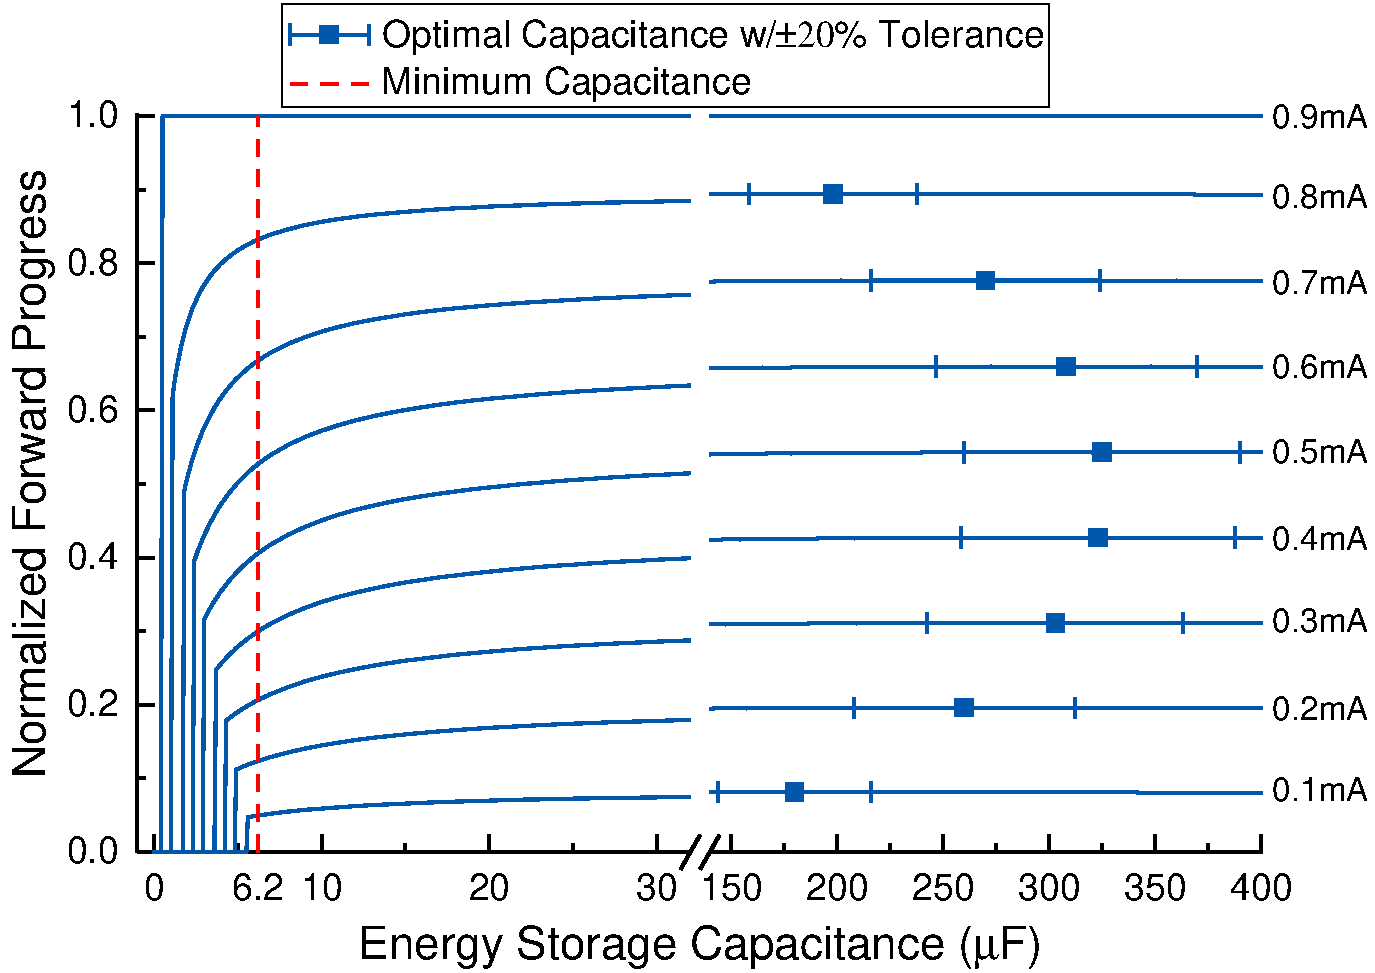
\includegraphics[width=3.2in]{ch3_sizingeffect/figures/StorCCur6Fig} 
  \caption{Forward progress against energy storage capacitance at different levels of constant supply current. Error bars around optimal points denote the impact of typical $\pm$20\% capacitance tolerance. }
  \label{fig:fpwconstcurr}
\end{figure}

\begin{figure}[!t]
  \centering
  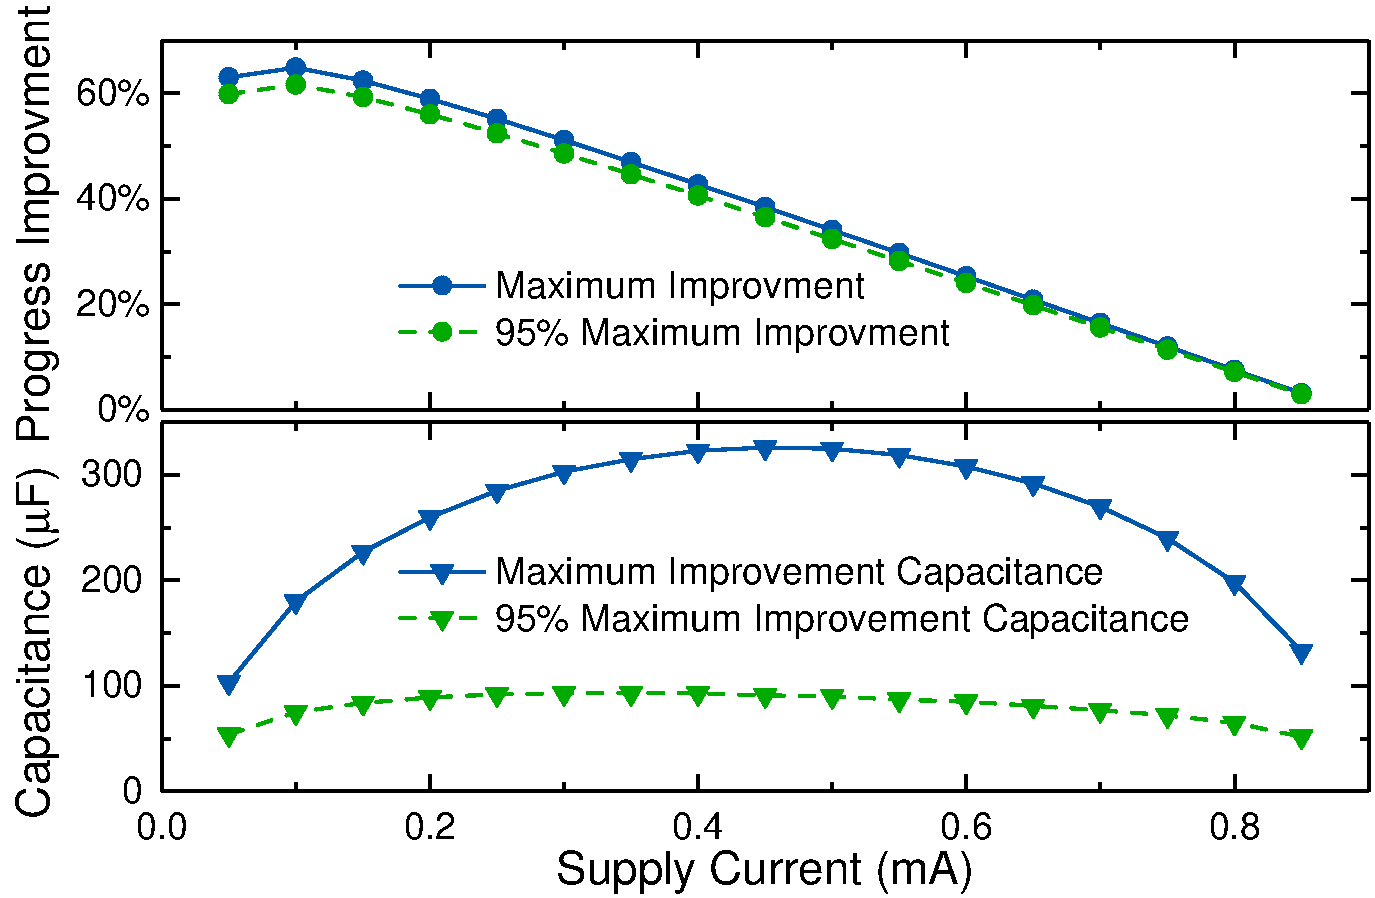
\includegraphics[width=3.2in]{ch3_sizingeffect/figures/StorCCurMax4Fig}
  \caption{Maximum forward progress improvement by sizing energy storage given a spectrum of supply current (normalized by the minimum capacitance case), with the corresponding maximum and sub-maximum (95\% of maximum) capacitance. }
  \label{fig:maxfwp}
\end{figure}

\figurename{~\ref{fig:maxfwp}} shows that an improvement in forward progress of up to 65\%  can be achieved when using the optimal capacitance instead of the minimum. However, it may not be desirable to set the capacitance solely for maximizing forward progress, because there are often trade-offs with other factors including increased interruption periods and dimensions. 
% (explored in Section~\ref{subsec:tradeoff}).
% In real-world energy source conditions, the supply current varies across this spectrum, and hence leads to an overall progress improvement based on its supply distribution. 
% This improvement exists only when the device operates in the Intermittent mode, since the device keeps either inactive in the Off mode or active in the On mode without the need for restoring and saving state. 
% Correspondingly, the optimal energy storage capacity is also plotted against supply current. 
% This optimal capacity exists because of the side effect of capacitor leakage; without capacitor leakage effect, the forward progress would keep approaching the ideal case (as explained in Section~\ref{subsec:formulation}). 
While a large improvement can be delivered with the optimal capacitance, as shown in \figurename{~\ref{fig:maxfwp}}, 95\% of this gain can still be obtained with significantly smaller capacitances (mean 31\% of the optimal value).
For example, reducing from \SI{325}{\micro\farad} to \SI{90}{\micro\farad} gives 95\% of the maximum improvement with a \SI{0.5}{\milli\ampere} supply. 

% in real deployment, storage fixed while current varies, change over a range, we may need to pick a capacity that optimise the majority of energy conditions. 

\subsubsection{Impact of Volatile State Size}

The size of volatile state differs across applications with different amounts of RAM usage, and hence incurs varying time and energy overheads for restore and save operations. We measured time overheads of restore and save operations in the minimum case (64B register data and a 160B stack) and the maximum case (64B register data and a full 2048B RAM) respectively as shown in Table~\ref{tab:ramscale}. As these time overheads are expected to be linear to the state size~\cite{Sliper:2019:ESR:3316781.3317812}, the model can be tuned for various volatile state sizes by linearly scaling the profiled values. 

% In the MCU we explore, volatile state includes CPU registers and SRAM data, which takes 64B and 160-2048B. 

\begin{table}[!t]
    \renewcommand{\arraystretch}{1.2}
    \centering
    \caption{Linear scaling range of volatile state size and restore/save time overheads}
    \label{tab:ramscale}
    \begin{tabular}{|c|cc|}
    \hline
    \textbf{State Size} & \multirow{2}{*}{\textbf{Restore Time}} & \multirow{2}{*}{\textbf{Save Time}}\\
    \textbf{(Registers + SRAM)} & & \\
    \hline
    64B + 160B (lower bound) & \SI{232}{\micro\second} & \SI{208}{\micro\second}\\
    % 64B registers + 160B stack
    64B + 2048B (upper bound) & \SI{2.298}{\milli\second} & \SI{2.274}{\milli\second} \\
    % 64B registers + 2048B RAM
    \hline
    \end{tabular}
\end{table}

An example of this is plotted in \figurename{~\ref{fig:ram}}. The forward progress improvement by sizing energy storage increases with the volatile state size, and the optimal capacitance grows accordingly. The improvement becomes insignificant when the volatile state size is small because the restore and save overheads are already negligible. For example, when the workload uses the least volatile state (the leftmost point), the maximum progress improvement is only 3.6\% although the restore and save overheads are reduced by 93\%. 
% This indicates the more efficiently ICSs save/restore, the more useless this work is. 

\begin{figure}[!t]
    \centering
    \includegraphics[width=3.2in]{ch3_sizingeffect/figures/RSTORAM3Fig}
    \caption{Impact of RAM usage (linear to restore/save overheads) on sizing energy storage with \SI{0.4}{\milli\ampere} current supply. Improvement and reduction are normalized by the minimum capacitance case. }
    \label{fig:ram}
\end{figure}
   
\section{Sizing under Real-World Energy Conditions} \label{sec:c4_demo}

In this section, we model an IPS with a PV energy harvester to explore the energy storage sizing effect in real-world energy conditions, and demonstrate use of the proposed sizing approach. 

\begin{figure}
    \centering
    \includegraphics[width=\columnwidth]{ch4_sizingapproach/figures/solarmodel4}
    \caption{System model of a PV-based IPS.}
    \label{fig:Model}
\end{figure}

\subsection{Simulation Configuration}

We integrate the validated reactive IPS model into a system model with a PV energy-harvesting supply as shown in \fref{fig:Model}. 
The energy storage model and the intermittent load model are as presented in \sref{sec:c3_exploration}. 

We use a converter-less supply circuit where only a Schottky diode is connected to the energy harvester output in order to prevent current backflow. 
The energy source conditions are imported from NREL outdoor solar irradiance data~\cite{stoffel1981nrel} and EnHANTs indoor irradiance data~\cite{6244798}. 
Four sets of light conditions are used to encompass different energy environments. 
To convert irradiance into harvested power, we adopt a PV cell model~\cite{en9050326} which uses the parameters available in common datasheets, so it can easily be reconfigured to suit various devices. 
The output current \nm{I}{o} of the PV cell model can then be described as:
\begin{equation} \label{eq:pvcell}
    \nmm{I}{o} = \frac{G}{\nmm{G}{ref}} \nmm{I}{sc} (1 - (1 - \frac{\nmm{I}{mpp}}{\nmm{I}{sc}}) ^ {\frac{\nmm{V}{o}-\nmm{V}{oc}}{\nmm{V}{mpp} - \nmm{V}{oc}}})
\end{equation}
where \nm{V}{o} is the output voltage of the PV cell, $G$ is the ambient irradiance, \nm{G}{ref} is the reference irradiance (normally \SI{1000}{\watt\per\square\centi\meter}), and \nm{I}{sc}, \nm{V}{oc}, \nm{I}{mpp}, \nm{V}{mpp} are respectively short-circuit current, open-circuit voltage, and the current and voltage at maximum power point (MPP) given the reference irradiance. 
\nm{V}{o} and $G$ are dynamic at run time, while other parameters in this model are constant. 
We refer to Panasonic Amorton glass type solar cells~\cite{solarcell} for PV cell properties as shown in \tref{tab:pvcell}. 
We set four cells in series (with \nm{V}{oc} = 3.56V) to match the operating voltage of the MCU (maximum 3.6V), and model energy harvester sizing by scaling the cell area. 


% A PV panel is an array of PV cells, which amplifies voltage and current output by connecting PV cells in series or parallel. In a PV panel, the open-circuit voltage is proportional to the number of cells in series, and the short-circuit current is proportional to the area of each cell and the number of cells in parallel. 

\begin{table}
    \renewcommand{\arraystretch}{1.2}
    \centering
    \begin{tabular}{|c|c|}
    \hline
    \textbf{Parameter} & \textbf{Value}\\
    \hline
    Open-Circuit Voltage & \SI{0.89}{\volt}/cell\\
    Short-Circuit Current & \SI{14.8}{\milli\ampere\per\square\centi\meter}\\
    Maximum Power Voltage & \SI{0.65}{\volt}/cell\\ 
    Maximum Power Current & \SI{12.1}{\milli\ampere\per\square\centi\meter}\\
    \hline
    \end{tabular}
    \caption{PV cell properties under a \SI{1000}{\watt\per\square\centi\meter}, AM-1.5 light source.}
    \label{tab:pvcell}
\end{table}

Our simulation tool can perform two simulation processes: (a) sort and process the time distribution of environmental conditions, and (b) simulate system state chronologically with a fine-grained time step. 
Process (a) reduces simulation time significantly, e.g. from hours to seconds, but ignores the restore operation after a brownout reset, hence overestimating forward progress, and it overestimates more with smaller capacitance and lower supply current. 
In the following results, \fref{fig:harvstor} comes from Process (a) for fast exploration, and \fref{fig:interruption} and \fref{fig:tradeoff} come from Process (b) for accurate records of interruption periods. 

\subsection{Exploration with Real-World Energy Source Conditions} \label{subsec:harvstor}

% Goal: 
% 1. to show that this model can help designers to find a suitable size of EH to achieve their desired performance;
% 2. to show that sizing energy storage would have different degrees of impact on real deployment depending on the specific energy conditions;
% 3. demonstrate sizing approach. 

In real-world deployments, ambient energy source conditions are dependent on time and location. 
The energy harvester and storage need to be sized to achieve the desired forward progress across the range of expected conditions. 

\subsubsection{Sizing the Energy Harvester}

For the purposes of this exploration, three levels of baseline mean forward progress (\nm{\alpha}{exe}) are set as 0.1, 0.2, and 0.3. 
We use the system model to find the PV panel area that achieves the expected forward progress under the different energy source conditions with minimum energy storage. 
We scale the PV panel area to find that which achieves each baseline \nm{\alpha}{exe}. 
As shown in \fref{fig:harvstor}, the energy harvester sizes that achieve the desired \nm{\alpha}{exe} may span orders of magnitude given different energy source conditions from \SI{}{\square\milli\meter} for outdoor sources ((c) and (d)) to \SI{}{\square\centi\meter} for indoor sources ((a) and (b)).  

\subsubsection{Sizing the Energy Storage}

Having obtained the energy harvester sizes for the baseline forward progress, we then use the modelling approach to size energy storage.
% A table lists the PV panel area to achieve the target \nm{\alpha}{exe} with minimum energy storage capacitance, the optimal capacitance with the forward progress improvement, and the alternative (decreased) PV panel area with the optimal capacitance. 
We analyse the sizing effect of energy storage on forward progress given real-world energy conditions. \fref{fig:harvstor} shows a 7.8-43.3\% improvement in forward progress by sizing energy storage under the given real-world energy conditions and baseline energy harvester sizes. 
It can also be inferred that optimising energy storage can either improve forward progress for a given energy harvester size, or reduce the energy harvester size that achieves the target forward progress. 
Given higher-power energy sources (e.g. Denver 2018 and Hawaii 2018 outdoor solar), increasing the harvester size efficiently improves forward progress with minor dimensional overheads, e.g. tens of \SI{}{\square\milli\meter}; however, given lower-power sources (e.g. EnHANTs Setup~A and Setup~D indoor light), optimising energy storage capacitance can save tens of \SI{}{\square\centi\meter} of PV panel area to achieve the same forward progress.

Also, the progress improvement by sizing energy storage varies accordingly with energy source conditions. 
As mentioned in \cref{chapter:sizingeffect}, this improvement stems from the reduction of restore and save overheads when the supply current is low and the device work in the \textit{Intermittent} mode. 
Thus, the results of EnHANTs Setup~A and Setup~D show a higher progress improvement from sizing energy storage than those of Denver 2018 and Hawaii 2018. 

\begin{figure}
    \centering
    \begin{subfigure}{0.51\columnwidth}
        \centering
        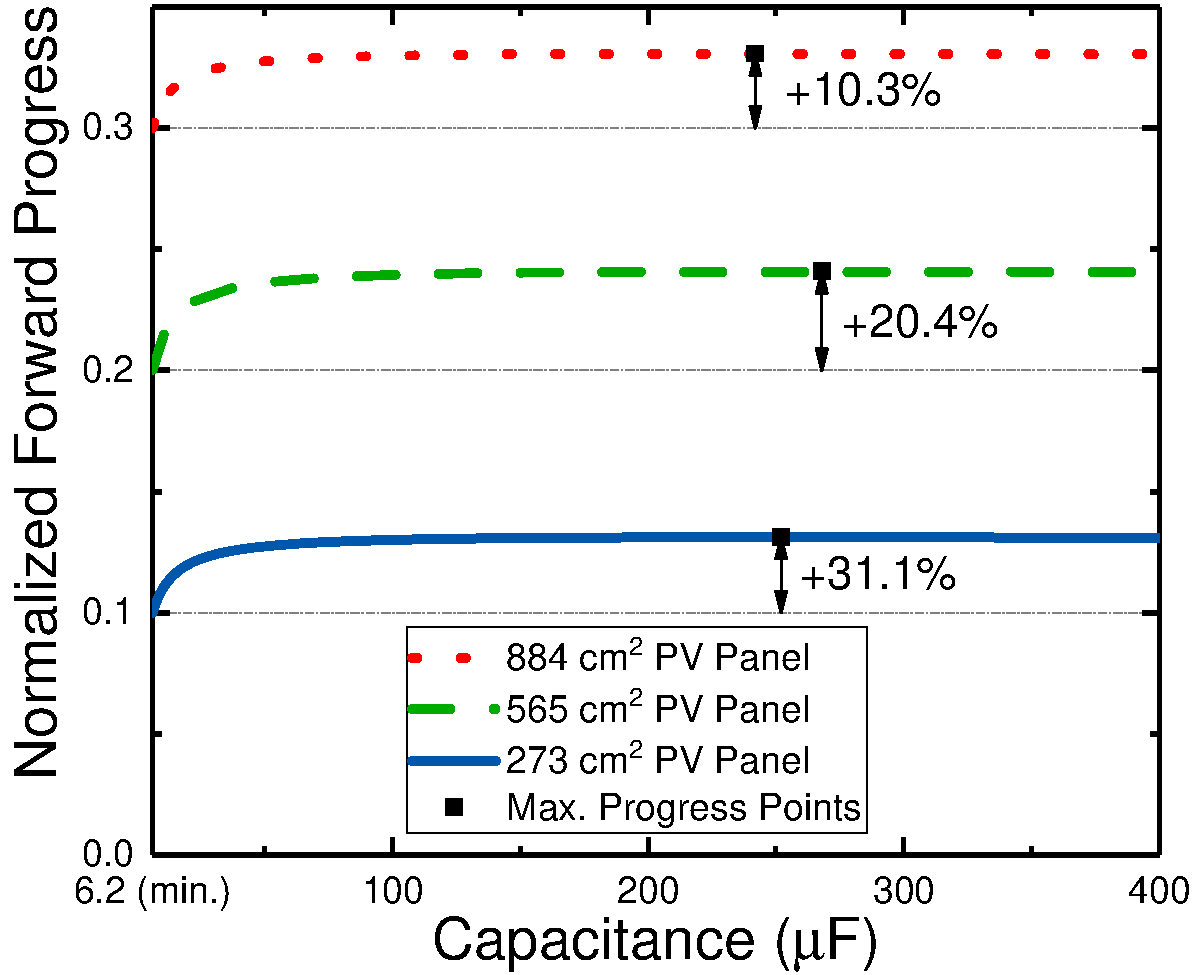
\includegraphics[width=\columnwidth]{ch4_sizingapproach/figures/HarvStorTgFig1}
        \caption{EnHANTs Setup A}
        \label{fig:harvstor1}
    \end{subfigure}
    \begin{subfigure}{0.483\columnwidth}
        \centering
        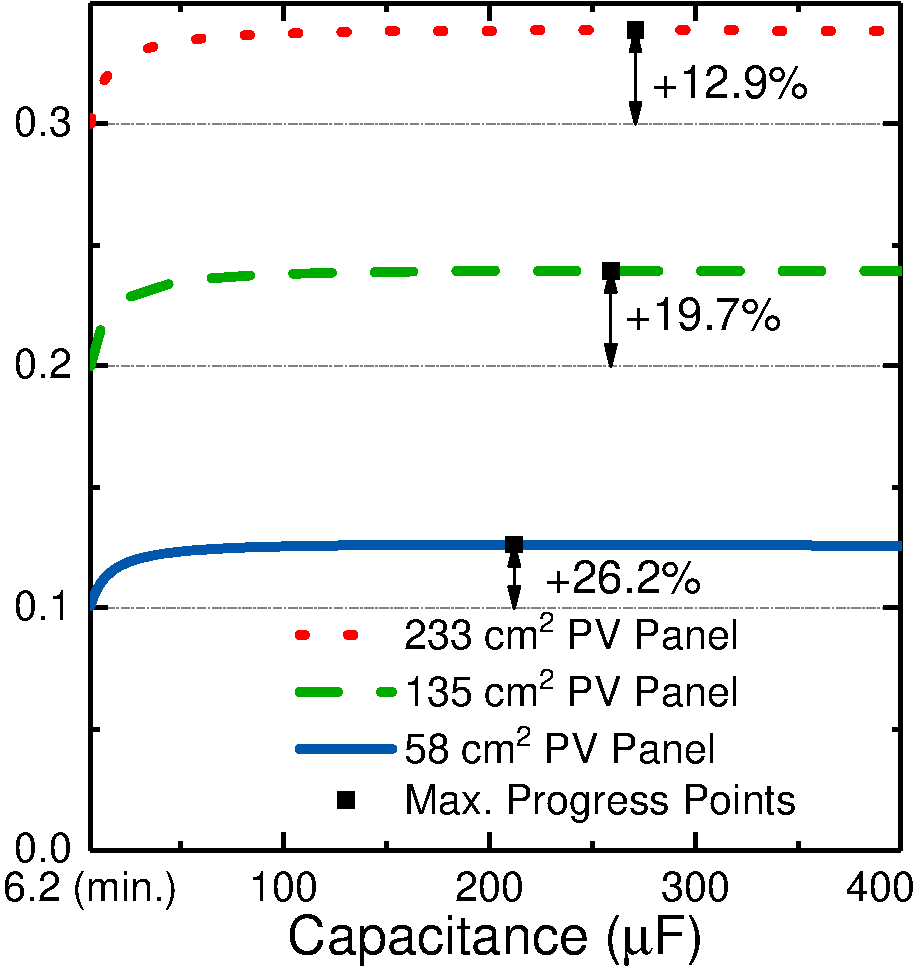
\includegraphics[width=\columnwidth]{ch4_sizingapproach/figures/HarvStorTgFig2}
        \caption{EnHANTs Setup D}
        \label{fig:harvstor2}
    \end{subfigure}
    \hfil
    \begin{subfigure}{0.51\columnwidth}
        \centering
        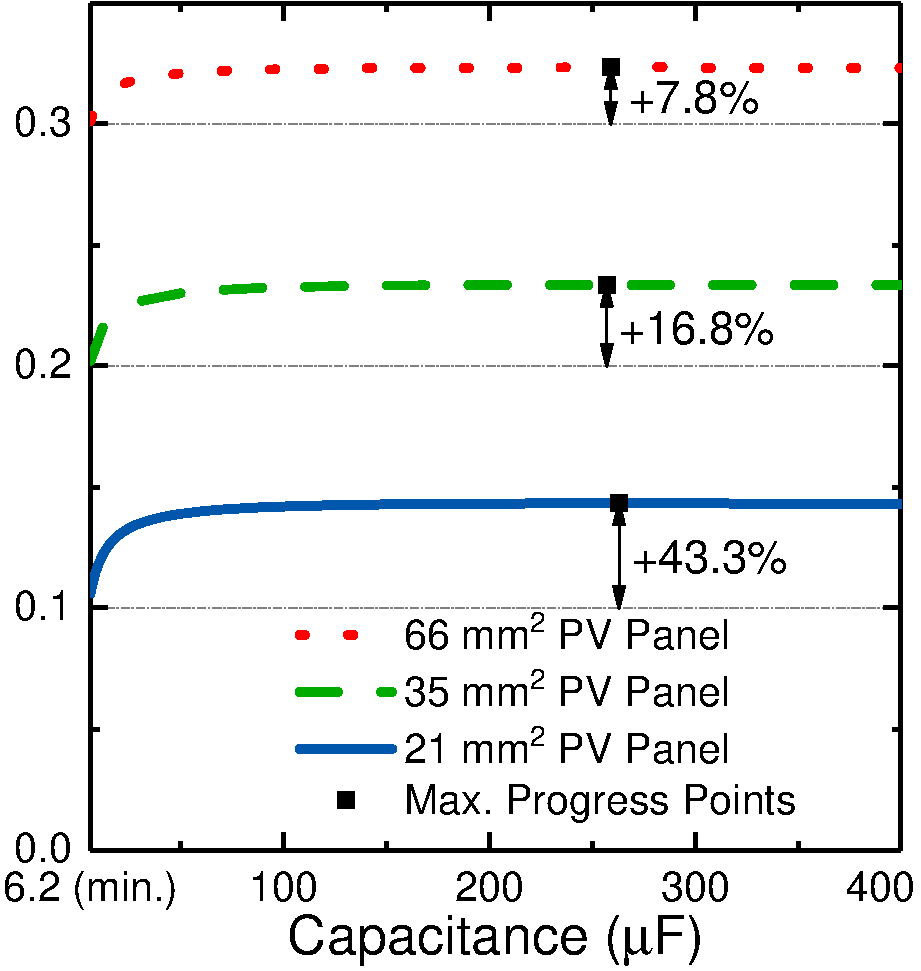
\includegraphics[width=\columnwidth]{ch4_sizingapproach/figures/HarvStorTgFig3}
        \caption{NREL Denver 2018}
        \label{fig:harvstor3}
    \end{subfigure}
    \begin{subfigure}{0.483\columnwidth}
        \centering
        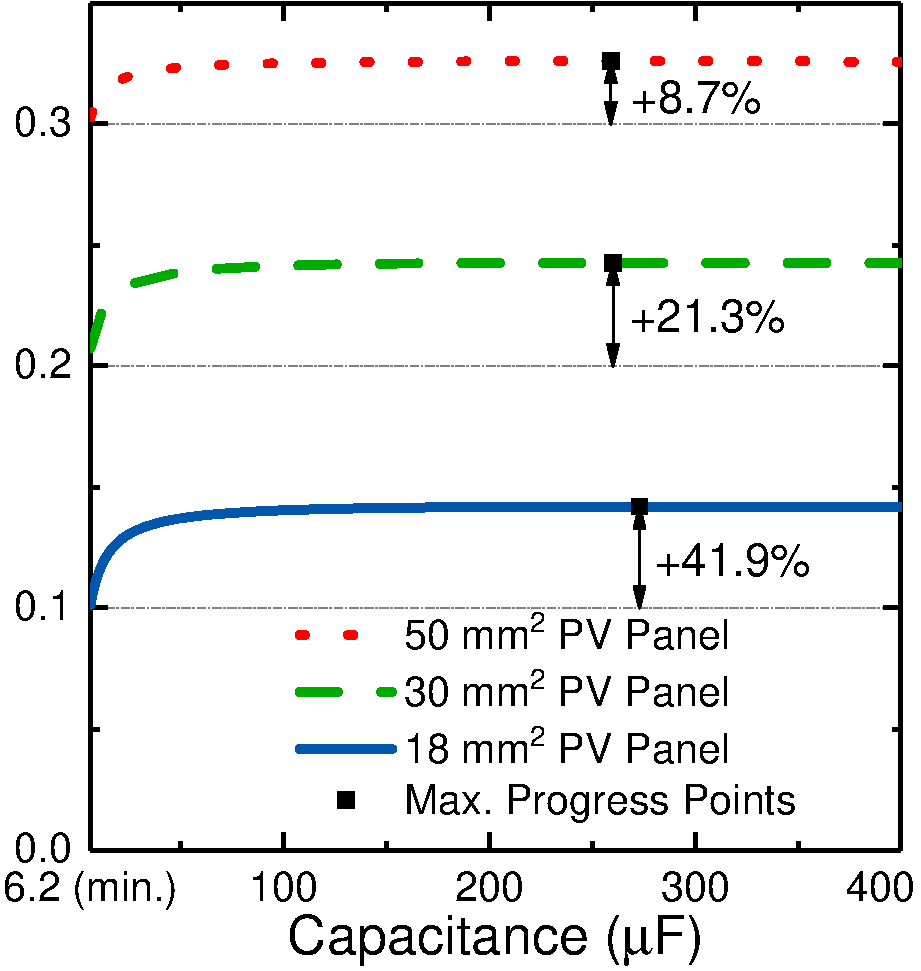
\includegraphics[width=\columnwidth]{ch4_sizingapproach/figures/HarvStorTgFig4}
        \caption{NREL Hawaii 2018}
        \label{fig:harvstor4}
    \end{subfigure}
    \caption{Improvement of average forward progress by sizing energy storage given different PV panel areas under real-world energy source conditions. The model is able to find the PV panel area required for achieving the target mean forward progress. } 
    \label{fig:harvstor}
\end{figure}

The mean forward progress given target \nm{\alpha}{exe} = 0.1 is plotted in \fref{fig:harvstorrange}, with the 60th and 90th time percentiles of forward progress. In all the  above datasets, the energy source is absent and the system is off for around \SI{55}{\percent} of time, so we plot the percentiles from the 60th. The mean progress during the energy-available periods is averaged over the energy-absent periods, so the actual mean forward progress during the energy-available periods is nearly double the annual mean. 

% Absolute improvement are different? Large variations? What other results can I add? 
% The variations of forward progress are significant due to the large variations of energy source conditions, so practical implementation should consider such variation as .
% The improved progress during the energy-available periods is averaged over the energy-absent periods, so the actual amount of improvement when energy is available is higher than the mean. (wrong statement)

\begin{figure}
    \centering
    \begin{subfigure}{0.51\columnwidth}
        \centering
        \includegraphics[width=\columnwidth]{ch4_sizingapproach/figures/HarvStorRan2Fig1}
        \caption{EnHANTs Setup A}
        \label{fig:harvstorrange1}
    \end{subfigure}
    \begin{subfigure}{0.483\columnwidth}
        \centering
        \includegraphics[width=\columnwidth]{ch4_sizingapproach/figures/HarvStorRan2Fig2}
        \caption{EnHANTs Setup D}
        \label{fig:harvstorrange2}
    \end{subfigure}
    \hfil
    \begin{subfigure}{0.51\columnwidth}
        \centering
        \includegraphics[width=\columnwidth]{ch4_sizingapproach/figures/HarvStorRan2Fig3}
        \caption{NREL Denver 2018}
        \label{fig:harvstorrange3}
    \end{subfigure}
    \begin{subfigure}{0.483\columnwidth}
        \centering
        \includegraphics[width=\columnwidth]{ch4_sizingapproach/figures/HarvStorRan2Fig4}
        \caption{NREL Hawaii 2018}
        \label{fig:harvstorrange4}
    \end{subfigure}
    \caption{Time percentiles of forward progress by sizing energy storage with target \nm{\alpha}{exe} = 0.1 and the corresponding PV panel area listed in \fref{fig:harvstor}. The percentiles start from the 60th as the system is off for around \SI{55}{\percent} of time due to insufficient energy source. }
    \label{fig:harvstorrange}
\end{figure}

\subsubsection{Interruption Period} \label{subsubsec:intper}
Besides forward progress, we also explore how the capacitance can change the interruption periods. 
When interrupted by insufficient power supply, an IPS enters an interruption period where it saves its volatile state, waits for supply voltage to recover, and restores the state to resume execution, without making any forward progress. 
Applications that require frequent sensing may be negatively affected by long interruption periods. 
We measure an interruption period as \textit{the period between two successive execution periods}, e.g. a consecutive `SLR' period in \fref{fig:operatingCycle} forms an interruption period. 
We record all the interruption periods during a one-year simulation with \SIrange{10}{50}{\micro\farad} capacitors, the Denver 2018 dataset, and an \SI{80}{\square\milli\meter} PV panel. 
\fref{fig:interruption} presents the distribution of all the interruption periods. 
With increased energy storage, the interruption period is prolonged. 
For example, the 90th percentile of interruption periods increases from \SI{32.2}{\milli\second} at \SI{10}{\micro\farad} to \SI{123.4}{\milli\second} at \SI{50}{\micro\farad} at an approximate rate of \SI{23}{\milli\second} per \SI{10}{\micro\farad}. 
% The majority of the interruption periods are within \SI{200}{\milli\second}. 
Facilitated by the simulator, developers are enabled to estimate whether the distribution of interruption periods meet their application requirement. 

% Whether and how much this would affect  Time-sensitive applications may care 
% the total number of interruptions is reduced,


\begin{figure}
    \centering
    \includegraphics[width=\columnwidth]{ch4_sizingapproach/figures/IntPeriodOrdFig}
    \caption{Distribution of interruption periods. }
    \label{fig:interruption}
\end{figure}

\subsection{Trading Forward Progress, Dimensions, and Interruption Period} \label{subsec:tradeoff}

Although increasing energy storage capacitance improves forward progress, larger capacitance increases both dimensions and interruption periods. 
We evaluate the overheads of increased capacitor dimensions and interruption periods, and then trade them off against forward progress using a cost function to suggest an optimal capacitance value. 

\subsubsection{Metric of Dimensions}

The overhead of capacitor dimensions is evaluated by characteristics of off-the-shelf tantalum capacitors. 
We narrow down the range of sample capacitors within a set of characteristics: low-profile, 10V rated voltage, and surface-mount package, and select six series of capacitors\footnote{The series of capacitor considered were: AVX TAJ, AVX TACmicrochip, AVX F92, Vishay 572D, Vishay 591D, and Vishay 592D.}. 
The volume and capacitance of these devices are plotted in \fref{fig:capvol}. 
We use the regression of these data to approximate a capacitance-volume relationship.
% ~\cite{tancap1, tancap2, tancap3, tancap4, tancap5, tancap6}
% Among the common capacitor chemistries with \textmu F to mF capacitance, tantalum capacitors manifest low leakage 

\begin{figure}
    \centering
    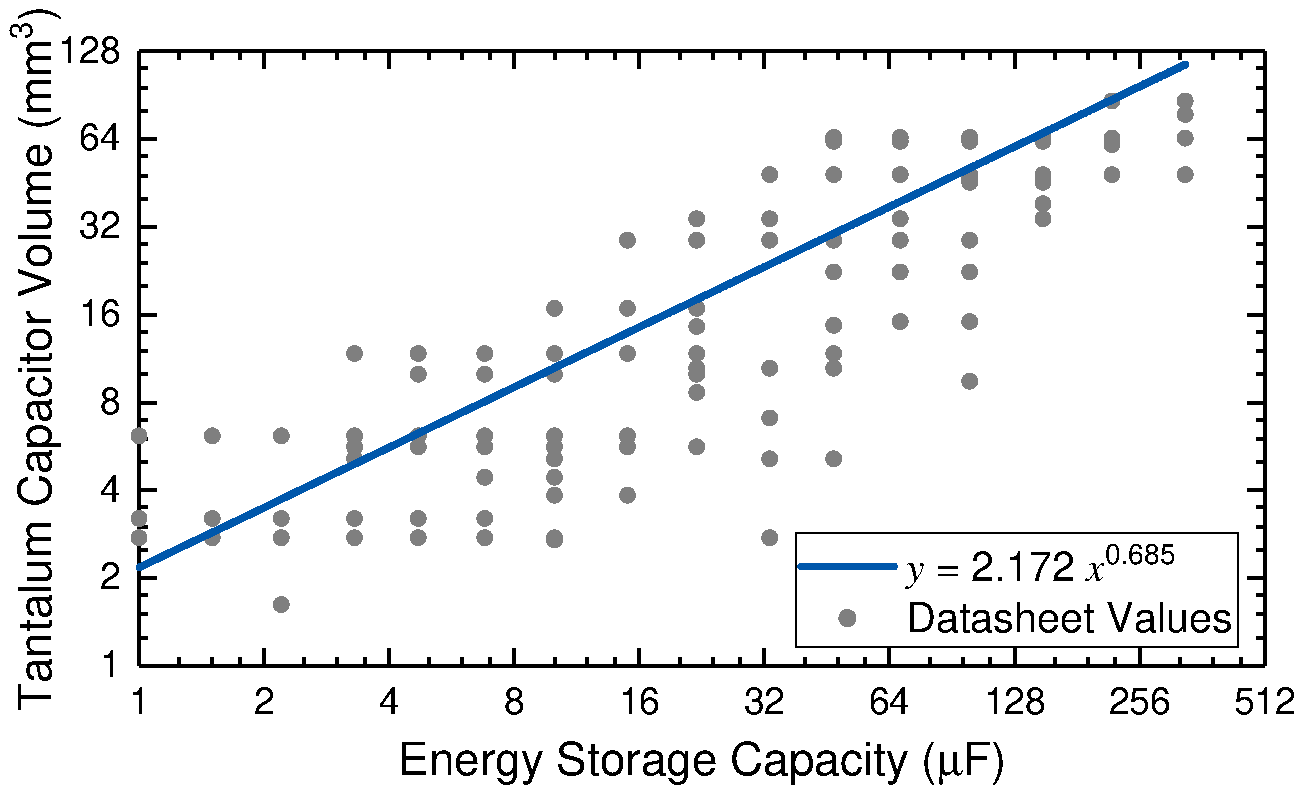
\includegraphics[width=\columnwidth]{ch4_sizingapproach/figures/CapVol2Fig2}
    \caption{Tantalum capacitor volume against capacitance for the six series of capacitors analysed. }
    \label{fig:capvol}
\end{figure}

\subsubsection{Metric of Interruption Periods} \label{subsubsec:metricintper}

% Definition/Measurement of interruption periods. recharging ability? Considering leakage?
% why interruption periods is important, why we consider it.

% , i.e. the period that does not make forward progress. The total interruption periods should be opposite to forward progress. 
Applications may have various requirements on interruption periods. 
To demonstrate the usage of our sizing approach, we consider a designer requests the 90th percentile of all interruption periods as an example metric of interruption periods, denoted as \nm{T}{int}. 
This metric indicates 90\% of interruption periods are shorter than \nm{T}{int}. 
This metric can be adapted for particular application requirements. 
% In We assume that $T_{interrupt}$ is preferable to be short for general application. 

\subsubsection{Cost Function}

From the previous observations (\fref{fig:maxfwp}) we can see that achieving the optimal progress improvement costs much more capacitance (mean 3.2$\times$) than to achieve 95\% improvement. 
A trade-off is necessary to improve forward progress while restricting the overheads of increased capacitor volume and interruption periods. 
This involves a problem of multi-criteria decision making~\cite{triantaphyllou2000multi}, which is outside the scope of this work. 
Nevertheless, we provide a cost function in (\ref{eq:tradeoff}) as an example to illustrate how these three factors could be traded-off, but designers are expected to customise a cost function with parameters of importance to specific application requirements. 
Note that the function (\ref{eq:tradeoff}) is to be maximised to find the recommended capacitance. 
\begin{equation}
    f = \frac{\nmm{\alpha}{exe}}{\nmm{k}{1}} - \left(\frac{\nmm{v}{cap}}{\nmm{k}{2}}\right) ^ {2} - \left(\frac{\nmm{T}{int}}{\nmm{k}{3}}\right) ^ {2} 
    \label{eq:tradeoff}
\end{equation}
\nm{\alpha}{exe} denotes normalised forward progress, \nm{v}{cap} denotes capacitor volume, and \nm{T}{int} denotes application interruption periods as mentioned in \sref{subsubsec:metricintper}. 
\nm{\alpha}{exe}, \nm{v}{cap}, and \nm{T}{int} can be generated from the simulation tool given $C$ as an input. 
\nm{k}{1}, \nm{k}{2}, and \nm{k}{3} are coefficients for normalising each metric, and they are empirically determined according to applications. 
In this example, the undesirable parameters are expressed as quadratic and negative terms to give an increasing cost to higher values. 
While only three parameters are considered here, others (such as the energy harvester size) could be included for a system-wise sizing scenario.
As an example to demonstrate its usage, we arbitrarily configure the function by setting \nm{k}{1} = 0.2, \nm{k}{2} = \SI{200}{\cubic\milli\meter}, and \nm{k}{3} = \SI{500}{\milli\second}. 
%, i.e.:
%\begin{equation}
%    f = \frac{\nmm{\alpha}{exe}}{0.2} - (\frac{\nmm{v}{cap}}{200}) ^ {2} - T_{recharge} ^ {2} 
%    \label{eq:tradeoffuse}
%\end{equation}
% where \nm{v}{cap} is in \SI{}{\cubic\milli\meter} and $T_{recharge}$ is in second. Here, $\frac{1}{\nmm{k}{1}} / \frac{1}{\nmm{k}{2}}$ equals 1000, but this does not mean that forward progress is 1000 times more important than capacitor volume.

\subsubsection{Results}

The effect of the trade-off is plotted in \fref{fig:tradeoff} using the Denver 2018 energy source dataset. 
Compared to the capacitor size that solely maximises forward progress, on average, an appropriately-sized capacitor achieves 93\% of the maximum forward progress, while saving 83\% of capacitor volume and 91\% of interruption periods. 
This also demonstrates the efficacy of the cost function and the chosen coefficients. 
Compared to the minimum storage case, the appropriately-sized capacitor improves forward progress by 12-124\% with energy storage increased from \SI{6.2}{\micro\farad} to \SI{30}{\micro\farad}.

\begin{figure}
    \centering
    \includegraphics[width=\columnwidth]{ch4_sizingapproach/figures/Tradeoff3Fig}
    \caption{The sizing approach trades off forward progress, capacitor volume, and interruption periods. The results are plotted against a range of PV panel area, given Denver 2018 energy source dataset. }
    \label{fig:tradeoff}
\end{figure}

As shown in \fref{fig:capvol}, the closest available capacitance that satisfies the \SI{6.2}{\micro\farad} minimum capacitance is \SI{6.8}{\micro\farad}, whereas the closest available capacitance to the appropriate \SI{30}{\micro\farad} is \SI{33}{\micro\farad}. 
The minimum volumes of \SI{6.8}{\micro\farad} and \SI{33}{\micro\farad} capacitors are both \SI{2.75}{\cubic\milli\meter}, which means using the appropriate capacitance, instead of the minimum one, may not incur dimensional overhead. 
% For \SI{47}{\micro\farad}, the absolute volume (\SI{5.12}{\cubic\milli\meter}) is insignificant compared to the device as a whole, e.g. an MSP430FR6989 MCU chip alone occupies \SI{274.4}{\cubic\milli\meter} (14 $\times$ 14 $\times$ 1.4). 
The regressed volume of the above two capacitance values are \SI{8.1}{\cubic\milli\meter} and \SI{23.8}{\cubic\milli\meter} respectively. 
However, the selection of capacitors can be dependent on factors other than physical volume, such as reliability, operation temperature, and more specific application needs. 
These factors can also be added into the cost function if necessary. 
% Again, such a volume scale is still insignificant in a whole device. 

            


\section{Conclusions} \label{section:conclusion}

% We explored the relationship between forward progress and energy storage capacitance in intermittent computing through a theoretical model.

% In this paper, we presented a model of reactive ICSs that accurately estimates forward progress. 
% Using this model, we explored the sizing effect of energy storage on forward progress with respect to supply current and volatile state size, showing up to \SI{64.9}{\percent} progress improvement under constant current supply and \SIrange{7.8}{43.3}{\percent} improvement on annual mean forward progress 
% under various real-world energy conditions. 

While conventional ICSs have used minimal levels of capacitance, this paper has shown that increasing the amount of energy storage can improve system performance by up to 65\% with a constant current supply and 43\% with real-world PV sources. The work includes a simulation tool which is available to download, enabling researchers to experiment with energy storage sizes to optimize ICS designs. A cost function can be incorporated, allowing various aspects of system performance to be traded-off. Our conclusion is that energy storage should be carefully designed, rather than minimized or indiscriminately picked, to efficiently operate ICSs.